%%
%% This is file `manuscript.tex',
%% generated with the docstrip utility.
%%
%% The original source files were:
%%
%% samples.dtx  (with options: `all,proceedings,manuscript')
%% 
%% IMPORTANT NOTICE:
%% 
%% For the copyright see the source file.
%% 
%% Any modified versions of this file must be renamed
%% with new filenames distinct from manuscript.tex.
%% 
%% For distribution of the original source see the terms
%% for copying and modification in the file samples.dtx.
%% 
%% This generated file may be distributed as long as the
%% original source files, as listed above, are part of the
%% same distribution. (The sources need not necessarily be
%% in the same archive or directory.)
%%
%%
%% Commands for TeXCount
%TC:macro \cite [option:text,text]
%TC:macro \citep [option:text,text]
%TC:macro \citet [option:text,text]
%TC:envir table 0 1
%TC:envir table* 0 1
%TC:envir tabular [ignore] word
%TC:envir displaymath 0 word
%TC:envir math 0 word
%TC:envir comment 0 0
%%
%% The first command in your LaTeX source must be the \documentclass
%% command.
%%
%% For submission and review of your manuscript please change the
%% command to \documentclass[manuscript, screen, review]{acmart}.
%%
%% When submitting camera ready or to TAPS, please change the command
%% to \documentclass[sigconf]{acmart} or whichever template is required
%% for your publication.
%%
%%
\documentclass[manuscript,screen,review]{acmart}
%%
%% \BibTeX command to typeset BibTeX logo in the docs
\AtBeginDocument{%
  \providecommand\BibTeX{{%
    Bib\TeX}}}

%% Packages for per-class category colour swatches (Tables 2a-c).
\usepackage[table]{xcolor}
\usepackage{colortbl}
\usepackage{multirow}

%% Reusable solid colour-swatch cell used inside the Class-Colour tables.
\newcommand{\clrsw}[1]{\textcolor{#1}{\rule{1.3em}{1.3ex}}}

%% Standard HSI benchmark palette (matches ground-truth maps printed by
%% matplotlib / standard HSI toolkits used across the baseline suite).
\definecolor{ipA}{RGB}{255,0,0}      \definecolor{ipB}{RGB}{0,255,0}
\definecolor{ipC}{RGB}{0,0,255}      \definecolor{ipD}{RGB}{255,255,0}
\definecolor{ipE}{RGB}{0,255,255}    \definecolor{ipF}{RGB}{255,0,255}
\definecolor{ipG}{RGB}{176,48,96}    \definecolor{ipH}{RGB}{46,139,87}
\definecolor{ipI}{RGB}{160,32,240}   \definecolor{ipJ}{RGB}{255,127,80}
\definecolor{ipK}{RGB}{127,255,212}  \definecolor{ipL}{RGB}{218,112,214}
\definecolor{ipM}{RGB}{160,82,45}    \definecolor{ipN}{RGB}{127,255,0}
\definecolor{ipO}{RGB}{216,191,216}  \definecolor{ipP}{RGB}{238,130,238}

%% Rights management information.  This information is sent to you
%% when you complete the rights form.  These commands have SAMPLE
%% values in them; it is your responsibility as an author to replace
%% the commands and values with those provided to you when you
%% complete the rights form.
\setcopyright{acmlicensed}
\copyrightyear{2018}
\acmYear{2018}
\acmDOI{XXXXXXX.XXXXXXX}
%% These commands are for a PROCEEDINGS abstract or paper.
\acmConference[Conference acronym 'XX]{Make sure to enter the correct
  conference title from your rights confirmation email}{June 03--05,
  2018}{Woodstock, NY}
%%
%%  Uncomment \acmBooktitle if the title of the proceedings is different
%%  from ``Proceedings of ...''!
%%
%%\acmBooktitle{Woodstock '18: ACM Symposium on Neural Gaze Detection,
%%  June 03--05, 2018, Woodstock, NY}
\acmISBN{978-1-4503-XXXX-X/2018/06}


%%
%% Submission ID.
%% Use this when submitting an article to a sponsored event. You'll
%% receive a unique submission ID from the organizers
%% of the event, and this ID should be used as the parameter to this command.
%%\acmSubmissionID{123-A56-BU3}

%%
%% For managing citations, it is recommended to use bibliography
%% files in BibTeX format.
%%
%% You can then either use BibTeX with the ACM-Reference-Format style,
%% or BibLaTeX with the acmnumeric or acmauthoryear sytles, that include
%% support for advanced citation of software artefact from the
%% biblatex-software package, also separately available on CTAN.
%%
%% Look at the sample-*-biblatex.tex files for templates showcasing
%% the biblatex styles.
%%
%%
%% The majority of ACM publications use numbered citations and
%% references.  The command \citestyle{authoryear} switches to the
%% "author year" style.
%%
%% If you are preparing content for an event
%% sponsored by ACM SIGGRAPH, you must use the "author year" style of
%% citations and references.
%% Uncommenting
%% the next command will enable that style.
%%\citestyle{acmauthoryear}


%%
%% end of the preamble, start of the body of the document source.
\begin{document}

%%
%% The "title" command has an optional parameter,
%% allowing the author to define a "short title" to be used in page headers.
\title[SGSCF-Net for HSI Classification]{SGSCF-Net: Spectral-Guided Spatial Cross-Attention Fusion Network for Hyperspectral Image Classification}

%%
%% The "author" command and its associated commands are used to define
%% the authors and their affiliations.
%% Of note is the shared affiliation of the first two authors, and the
%% "authornote" and "authornotemark" commands
%% used to denote shared contribution to the research.
\author{Tejas Surya}
\email{stkisan098.btech2023@it.nitrr.ac.in}
\affiliation{%
  \institution{National Institute of Technology (NIT) Raipur}
  \city{Raipur}
  \state{Chhattisgarh}
  \country{India}
}

\author{Author ABC}
\email{author.abc@institution.edu}
\affiliation{%
  \institution{Institute for Clarity in Documentation}
  \city{Dublin}
  \state{Ohio}
  \country{USA}
}

\author{Author XYZ}
\email{author.xyz@university.ac.uk}
\affiliation{%
  \institution{University of Advanced Research}
  \city{London}
  \country{United Kingdom}
}

%%
%% By default, the full list of authors will be used in the page
%% headers. Often, this list is too long, and will overlap
%% other information printed in the page headers. This command allows
%% the author to define a more concise list
%% of authors' names for this purpose.
\renewcommand{\shortauthors}{Surya et al.}

%%
%% The abstract is a short summary of the work to be presented in the
%% article.
\begin{abstract}
Hyperspectral image (HSI) classification is vital for remote sensing Earth observation. Although deep convolutional networks and vision transformers improve classification accuracy, they suffer from parameter redundancy, high computational latency, and vulnerability to atmospheric absorption noise. Conventional architectures also rely on first-order spatial pooling, discarding crucial high-order co-activation dependencies between spectral channels and spatial domains. To overcome these limitations without heavy transformer or state-space overheads, we propose the \textbf{Spectral-Guided Spatial Cross-Attention Fusion Network (SGSCF-Net)}. SGSCF-Net integrates three specialized modules: 
(1) a \textbf{Spectral Band Attention Module (SBAM)} operating on raw input bands before convolution to suppress noisy absorption channels; 
(2) a \textbf{Complementary Branch Spectral Attention (CBSA)} mechanism enforcing feature specialization between dual spectral-only ($1\times 1\times 7$) and spectral-spatial ($3\times 3\times 7$) 3D convolution streams via complementary gating; and 
(3) a \textbf{Second-Order Covariance Fusion Gate (SCFG)} capturing channel-spatial co-activation via bilinear outer-product covariance pooling. 
To protect decision boundaries on skewed land-cover distributions, training is governed by a minority-aware hybrid objective combining margin-scheduled Spread Loss and class-weighted Focal Loss. SGSCF-Net eliminates quadratic attention complexity while preserving rich representations. Benchmark evaluations on Indian Pines, Pavia University, and Salinas Valley demonstrate that SGSCF-Net reduces parameters and latency while matching or exceeding state-of-the-art accuracy, maintaining robust generalization even under severe sample scarcity.

\vspace{1.2ex}
\noindent\textbf{\textit{Index Terms}}---Hyperspectral image (HSI) classification, neural network, spectral-spatial attention, feature fusion.
\end{abstract}

%%
%% The code below is generated by the tool at http://dl.acm.org/ccs.cfm.
%% Please copy and paste the code instead of the example below.
%%
\begin{CCSXML}
<ccs2012>
 <concept>
  <concept_id>10010147.10010257.10010293.10010294</concept_id>
  <concept_desc>Computing methodologies~Neural networks</concept_desc>
  <concept_significance>500</concept_significance>
 </concept>
 <concept>
  <concept_id>10010147.10010178.10010224.10010245</concept_id>
  <concept_desc>Computing methodologies~Computer vision problems</concept_desc>
  <concept_significance>500</concept_significance>
 </concept>
 <concept>
  <concept_id>10010435.10010459.10010467</concept_id>
  <concept_desc>Applied computing~Environmental sciences</concept_desc>
  <concept_significance>300</concept_significance>
 </concept>
 <concept>
  <concept_id>10010147.10010257.10010258.10010259</concept_id>
  <concept_desc>Computing methodologies~Supervised learning by classification</concept_desc>
  <concept_significance>300</concept_significance>
 </concept>
</ccs2012>
\end{CCSXML}

\ccsdesc[500]{Computing methodologies~Neural networks}
\ccsdesc[500]{Computing methodologies~Computer vision problems}
\ccsdesc[300]{Applied computing~Environmental sciences}
\ccsdesc[300]{Computing methodologies~Supervised learning by classification}

\keywords{Hyperspectral Image Classification, Spectral-Spatial Feature Extraction, Attention Mechanism, Cross-Attention Fusion, Second-Order Covariance, Deep Learning}


\received{20 February 2007}
\received[revised]{12 March 2009}
\received[accepted]{5 June 2009}

%%
%% This command processes the author and affiliation and title
%% information and builds the first part of the formatted document.
\maketitle


\section{Introduction}
\label{sec:intro}
Hyperspectral image (HSI) acquisition captures continuous, narrow spectral bands across hundreds of contiguous wavelengths alongside rich two-dimensional spatial structures \cite{bioucas2012hyperspectral, plaza2009recent}. The resulting three-dimensional data cube provides a detailed diagnostic spectral signature for every spatial pixel, frequently referred to as a spectral fingerprint \cite{fauvel2012advances, ghamisi2017advanced}. By revealing subtle chemical and physical material properties imperceptible to standard trichromatic RGB sensors, HSI technology serves as a cornerstone in Earth observation. It is widely deployed across precision agriculture, ecological monitoring, mineral exploration, and urban surveyance.

HSI classification aims to assign a distinct land-cover semantic label to each spatial pixel by simultaneously interpreting complex spectral-spatial correlations. In recent years, deep learning models have emerged as the dominant paradigm for HSI classification \cite{chen2014deep, zhao2016spectral}. Specifically, convolutional neural networks (CNNs), particularly 3D CNNs and hybrid 2D-3D frameworks such as SSRN \cite{zhong2017spectral} and HybridSN \cite{roy2020hybridsn}, extract localized spectral-spatial features by applying learnable 3D kernel operations directly over contiguous bands, establishing a theoretical foundation for 3D volumetric convolution \cite{ben2018deep} built upon deep residual principles \cite{he2016deep}. However, cascading deep multi-scale 3D convolutional layers \cite{he2018multi} rapidly inflates parameter counts, precipitating substantial memory consumption and extended training latencies, while struggling to preserve complex parcel boundaries and diverse region structures across heterogeneous agricultural scenes \cite{zhang2018diverse}.

To overcome the local receptive field constraints of CNNs, Vision Transformers (ViTs) \cite{dosovitskiy2020image} and tokenized architectures such as HSI-SSFTT \cite{sun2022spectral}, Spatial-Spectral Transformer \cite{he2021spatial}, HiT \cite{yang2022hyperspectral}, and MorphFormer \cite{roy2023morphformer} have been introduced to capture global spatial-spectral dependencies via self-attention. However, standard self-attention mechanisms scale with quadratic computational complexity $\mathcal{O}(N^2)$ with respect to token sequence length. On dense HSI patches, this quadratic scaling imposes an acute computational bottleneck during both training and inference. Furthermore, hyperspectral data inherently suffer from non-uniform spectral noise, notably strong atmospheric water-vapor absorption bands. Most existing deep networks apply convolutional filters indiscriminately across all spectral bands without pre-filtering, allowing noise from uninformative bands to propagate into downstream latent representations. In addition, conventional architectures compress spatial dimensions using first-order global average pooling, discarding high-order co-activation statistics between specific spatial positions and discriminative spectral channels. Compounding these structural challenges, real-world HSI benchmarks feature severe class imbalance, where minority classes contain as few as tens of training samples, causing standard cross-entropy loss functions to experience catastrophic boundary collapse.

Rather than escalating model capacity through heavier Transformers or recurrent state-space models such as Mamba \cite{gu2023mamba}, an effective solution lies in targeted spectral gating and high-order covariance interaction. Unlike post-convolution attention blocks (e.g., CBAM \cite{woo2018cbam}) that recalibrate only after spatial blur has propagated, applying attention directly to raw input bands before any convolution enables the network to adaptively suppress noisy atmospheric channels at the earliest processing stage. Second, in dual-branch feature extractors combining spectral-only and joint spectral-spatial convolutions, enforcing a strictly complementary gating schedule ($\alpha$ versus $1-\alpha$) compels each stream to learn specialized, orthogonal representations rather than redundant features. Third, replacing first-order spatial pooling with second-order covariance pooling enables the model to capture fine-grained bilinear correlations between spatial activations and spectral channels without excessive parameter growth.

To this end, we design the \textbf{Spectral-Guided Spatial Cross-Attention Fusion Network (SGSCF-Net)}, an end-to-end framework tailored for efficient, noise-resilient hyperspectral classification. SGSCF-Net integrates three novel modules:
\begin{enumerate}
    \item \textbf{Spectral Band Attention Module (SBAM):} Positioned at the network entry, SBAM operates directly on raw spectral channels prior to convolution. It adaptively recalibrates input channels via a spatial-squeeze MLP bottleneck, attenuating uninformative absorption bands early.
    \item \textbf{Complementary Branch Spectral Attention (CBSA):} Across the dual 3D entry streams (a $1\times 1\times 7$ spectral branch and a $3\times 3\times 7$ spatial-spectral branch), CBSA computes a channel-wise gating parameter $\alpha \in (0, 1)$ via a lightweight depthwise 1D convolution. Fusing the branches as $\alpha \odot a + (1-\alpha) \odot b$ strictly enforces complementary feature specialization.
    \item \textbf{Second-Order Covariance Fusion Gate (SCFG):} After spectral feature compression, SCFG computes the outer product between global channel descriptors and spatial descriptors ($G = f_{\text{ch}} \otimes f_{\text{sp}}$), normalizing the resulting bilinear interaction tensor via Frobenius norm to gate spatial activations.
\end{enumerate}
To safeguard decision boundaries on skewed class distributions, SGSCF-Net is optimized using a minority-aware hybrid objective combining margin-scheduled Spread Loss \cite{sabour2018matrix} and class-weighted Focal Loss \cite{lin2017focal}, drawing upon margin optimization and sample-effective regularization principles \cite{cao2019learning, haut2021generative}. Containing approximately 308K parameters, SGSCF-Net operates with zero self-attention overhead while preserving high representational capacity.

The primary contributions of this work are summarized as follows:
\begin{enumerate}
    \item We introduce an input-level Spectral Band Attention Module (SBAM) that filters noisy and uninformative raw spectral bands prior to feature extraction, mitigating noise propagation throughout deeper layers.
    \item We formulate a Complementary Branch Spectral Attention (CBSA) mechanism that explicitly couples spectral-only and spatial-spectral 3D convolutions through complementary gating, ensuring optimal feature diversity without parameter inflation.
    \item We propose a Second-Order Covariance Fusion Gate (SCFG) that models bilinear channel-spatial co-activation, capturing fine-grained dependencies overlooked by standard first-order pooling operators.
\end{enumerate}

The remainder of this article is organized as follows. Section II provides a review of related literature across convolutional, attention-based, and transformer architectures for HSI classification. Section III presents the formal mathematical formulation of SGSCF-Net, detailing SBAM, CBSA, SCFG, and the hybrid training objective. Section IV reports the experimental setup, comparative baseline evaluations, and computational complexity analyses. Section V discusses ablation studies and data scarcity stress testing. Finally, Section VI concludes the paper.

\section{Related Work}
\label{sec:related_work}

\subsection{Convolutional Neural Networks for Hyperspectral Classification}
Deep learning models have substantially superseded conventional machine learning methods, such as support vector machines \cite{melgani2004classification} and kernel methods \cite{camps2005kernel}, by eliminating manual handcrafted feature engineering. Within this paradigm, convolutional neural networks (CNNs) have received widespread adoption for hyperspectral image (HSI) feature extraction \cite{chen2014deep, chen2016deep}. Early approaches focused on autoencoder architectures and one-dimensional CNNs (1D CNNs) to capture continuous spectral profiles across spectral curves \cite{chen2014deep, hu2015deep}. While effective at distinguishing fine spectral discrepancies, 1D CNNs entirely disregard the spatial context of adjacent pixels, making them susceptible to label noise in heterogeneous land covers.

To exploit spatial correlation, two-dimensional CNNs (2D CNNs) were subsequently adopted by applying spatial convolutions on principal-component-reduced bands \cite{zhao2016spectral}. However, spatial-only processing discards fine diagnostic spectral signatures across contiguous absorption bands. To overcome this limitation, three-dimensional convolutional neural networks (3D CNNs) were introduced to jointly extract spectral and spatial features directly from the raw volumetric HSI cube \cite{ben2018deep}. A prominent milestone is the Spectral-Spatial Residual Network (SSRN) \cite{zhong2017spectral}, which employs consecutive 3D residual blocks to learn joint spatial-spectral representations. Similarly, Roy \textit{et al.} proposed HybridSN \cite{roy2020hybridsn}, integrating cascaded 3D convolutions with downstream 2D convolutions to mitigate computational complexity. Furthermore, multi-scale 3D CNNs \cite{he2018multi} and diverse region-based CNNs \cite{zhang2018diverse} have explored multi-scale receptive field hierarchies to characterize spatial contextual variance across complex terrains.

Despite their success, standard 3D CNNs exhibit two critical shortcomings: (1) stacking multi-scale 3D convolutional kernels induces severe parameter explosion and quadratic memory overhead; and (2) existing CNN architectures apply kernels uniformly across all spectral channels without input-level pre-filtering, allowing strong atmospheric water-vapor noise to degrade deep representation learning.

\subsection{Attention Mechanisms, Vision Transformers, and State-Space Models}
To circumvent the localized receptive field constraint of standard convolution, attention mechanisms have been extensively investigated to dynamically weigh informative features. The Squeeze-and-Excitation Network (SENet) \cite{hu2018squeeze}, Convolutional Block Attention Module (CBAM) \cite{woo2018cbam}, and Efficient Channel Attention (ECA-Net) \cite{wang2020eca} introduced channel and spatial attention through global average pooling and local 1D convolutions. In remote sensing, Sun \textit{et al.} introduced the Spectral-Spatial Attention Network (SSAN) \cite{sun2019spectral}, which decouples attention into spatial and spectral branches. Subsequent architectures incorporated attention-aided CNNs \cite{hang2021hyperspectral}, residual attention mechanisms \cite{zhu2021residual}, and connected feature-grouped attention \cite{guo2022feature}. In parallel, reinforcement learning and attention strategies have been explored for explicit band selection and spectral channel weighting \cite{mou2022deep}. Furthermore, dual-branch frameworks such as the Attention-Based Adaptive Spectral-Spatial Kernel ResNet (A2S2K-ResNet) \cite{roy2020attention}, Double-Branch Dual-Attention Networks \cite{li2020double}, and CSCANet \cite{wang2023cscanet} utilize multi-branch streams to extract complementary spatial-spectral features. However, existing dual-branch frameworks frequently compute a single shared scalar weight or combine features via simple summation, failing to enforce feature specialization between the complementary streams.

Concurrently, Vision Transformers (ViTs) \cite{dosovitskiy2020image} have redefined computer vision by modeling long-range contextual relationships through multi-head self-attention. In hyperspectral remote sensing, architectures such as HSI-SSFTT \cite{sun2022spectral}, SpectralFormer \cite{hong2021spectralformer}, Spatial-Spectral Transformer \cite{he2021spatial}, HiT \cite{yang2022hyperspectral}, MorphFormer \cite{roy2023morphformer}, and improved Transformer variants \cite{qing2021improved} have achieved high classification accuracy by tokenizing spatial-spectral patches. Recently, state-space models such as Mamba \cite{gu2023mamba} and MambaHSI \cite{li2024mambahsi} have explored linear-complexity selective scan mechanisms. Nevertheless, self-attention mechanisms fundamentally incur quadratic computational complexity $\mathcal{O}(N^2)$ with respect to spatial-spectral token sequence length, leading to severe computational latency and hardware memory bottlenecks on dense HSI patches.

\subsection{Second-Order Covariance Representations and Class Imbalance}
A prominent limitation across conventional CNNs and Transformer backbones is their reliance on first-order statistics. Standard architectures compress spatial feature maps using Global Average Pooling (GAP), which calculates the arithmetic mean of spatial activations. While computationally trivial, GAP implicitly assumes spatial uniformity and discards crucial second-order co-activation statistics between spatial positions and spectral channels. In fine-grained computer vision, Bilinear CNNs \cite{lin2015bilinear} and global second-order pooling networks \cite{gao2019global, li2018towards} demonstrated that second-order outer-product covariance pooling captures rich co-occurrence statistics. In HSI classification, local covariance matrix representations \cite{fang2018new}, multiscale covariance maps \cite{he2019feature}, attention-based second-order pooling \cite{xue2021attention}, and mixed convolution covariance pooling \cite{zheng2021hyperspectral} confirmed the potency of covariance representations for capturing spatial-spectral correlations. Furthermore, capsule networks \cite{paoletti2018capsule} and Deep Matrix Capsules (DMC) with EM routing \cite{wang2021deep} incorporated high-order matrix poses to model spatial hierarchies, demonstrating high accuracy but requiring specialized routing iterations.

Compounding these architectural bottlenecks, hyperspectral benchmark datasets suffer from severe class imbalance. Certain agricultural categories (e.g., Oats in Indian Pines) possess as few as tens of samples, whereas dominant classes comprise thousands of samples. Standard cross-entropy loss gradients become heavily dominated by prevalent background classes, precipitating catastrophic boundary misclassifications on minority land covers. While Focal Loss \cite{lin2017focal} addresses hard-example mining through dynamic modulating factors, effective sample volume weighting \cite{cui2019class} and margin-based losses such as Spread Loss \cite{sabour2018matrix} and LDAM \cite{cao2019learning} enforce explicit margins between ground-truth activations and competing categories. In addition, minority oversampling techniques such as HyperGAMO \cite{haut2021generative} and feature-rotation ensembles \cite{su2023spectral} emphasize the necessity of safeguarding decision boundaries under extreme sample scarcity.

To reconcile these divergent challenges, \textbf{SGSCF-Net} introduces an integrated solution: (1) an input-level Spectral Band Attention Module (SBAM) that filters atmospheric absorption noise prior to convolution; (2) a Complementary Branch Spectral Attention (CBSA) mechanism that enforces orthogonal branch specialization through complementary gating ($\alpha$ vs $1-\alpha$); (3) a Second-Order Covariance Fusion Gate (SCFG) that models bilinear channel-spatial co-activation; and (4) a minority-aware hybrid objective combining margin-scheduled Spread Loss and Focal Loss. This yields state-of-the-art representation capacity with only $\sim$308K parameters and zero quadratic self-attention latency.

\section{Methodology}
\label{sec:methodology}
This section formalizes the mathematical architecture of SGSCF-Net. We first define the problem formulation and pipeline dataflow, followed by detailed formulations of SBAM (input band filtering), CBSA (orthogonal dual-branch fusion), SCFG (second-order covariance gating), and the minority-aware hybrid objective.

\subsection{Overall Pipeline and Problem Formulation}
\label{subsec:pipeline}
\begin{figure*}[t]
\centering
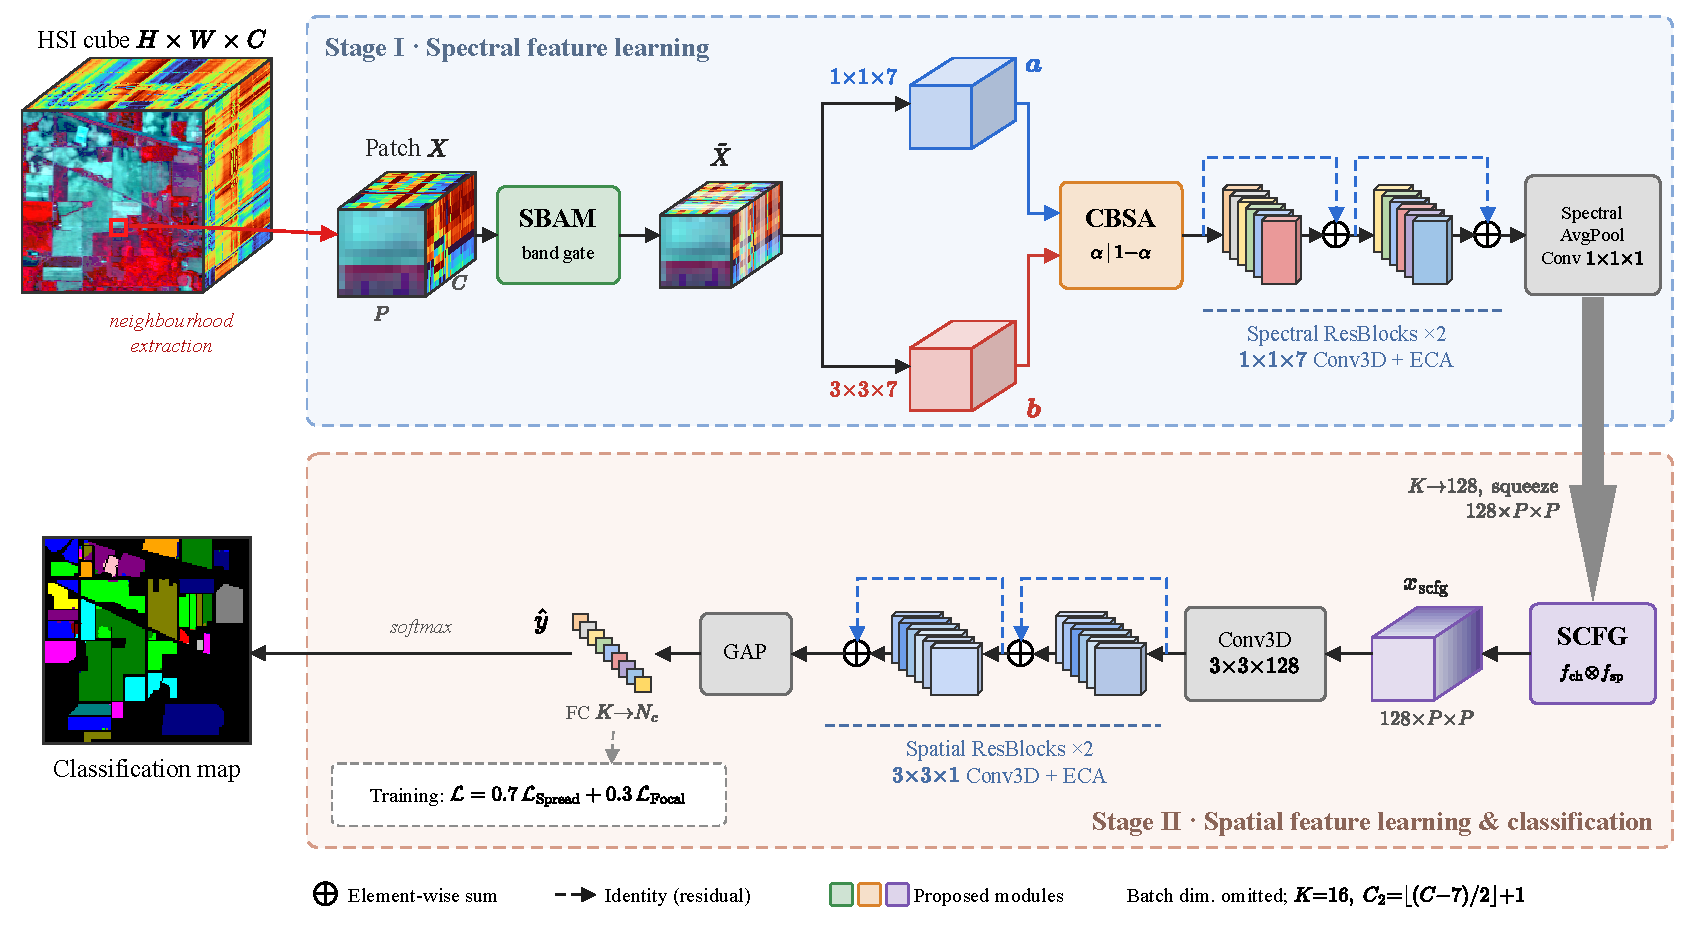
\includegraphics[width=0.98\textwidth]{figures/architecture/fig_sgscf_overall.pdf}
\caption{End-to-end architectural workflow of the proposed Spectral-Guided Spatial Cross-Attention Fusion Network (SGSCF-Net). The model processes raw hyperspectral cubes through two coordinated stages: Stage~I executes input-level spectral gating (SBAM) on raw patches and orthogonal dual-branch feature learning (CBSA) across spectral residual blocks; Stage~II performs spectral-to-spatial compression, second-order spatial-channel covariance fusion (SCFG), and spatial residual learning, concluding with Global Average Pooling (GAP) and minority-aware hybrid loss supervision.}
\label{fig:sgscf_overall}
\Description{End-to-end architectural workflow of SGSCF-Net across Stage I and Stage II.}
\end{figure*}

Let $\mathcal{X} \in \mathbb{R}^{H \times W \times C}$ denote the raw hyperspectral data cube, where $H$, $W$, and $C$ represent the spatial height, width, and number of contiguous spectral bands, respectively. Let $\mathcal{Y} \in \{1, 2, \dots, C_{\text{cls}}\}^{H \times W}$ denote the corresponding ground-truth land-cover semantic label map. For any labeled target pixel located at spatial coordinate $(i, j)$, we extract a localized spatial neighborhood cube of size $P \times P$ across all $C$ spectral channels. To handle boundary pixels, symmetric spatial reflection padding of size $p = \lfloor P / 2 \rfloor$ is applied. Each input sample is structured as a five-dimensional volumetric tensor:
\begin{equation}
\label{eq:input_tensor}
X \in \mathbb{R}^{B \times 1 \times P \times P \times C}
\end{equation}
where $B$ denotes the mini-batch size, and the unitary second dimension represents the input channel axis required for 3D convolutional operations.

The computational dataflow of SGSCF-Net, illustrated in Fig.~\ref{fig:sgscf_overall}, processes the input patch $X$ through two coordinated stages of spectral filtering and second-order spatial refinement. First, $X$ enters the \textbf{Spectral Band Attention Module (SBAM)} to produce an adaptively recalibrated tensor $\tilde{X} \in \mathbb{R}^{B \times 1 \times P \times P \times C}$, suppressing noisy atmospheric absorption channels before convolutional operations. Next, $\tilde{X}$ feeds into a \textbf{Dual 3D Entry Stream} that yields a spectral-only representation $a \in \mathbb{R}^{B \times K \times P \times P \times C_2}$ via $1\times 1\times 7$ convolution and a joint spatial-spectral representation $b \in \mathbb{R}^{B \times K \times P \times P \times C_2}$ via $3\times 3\times 7$ convolution, with $K=16$ filters and $C_2 = \lfloor(C-7)/2\rfloor + 1$. The \textbf{Complementary Branch Spectral Attention (CBSA)} mechanism then couples both streams using a depthwise 1D gate $\alpha \in \mathbb{R}^{B \times K \times 1 \times 1 \times C_2}$, fusing them as $\alpha \odot a + (1-\alpha) \odot b$ to enforce orthogonal feature specialization. The coupled tensor subsequently traverses two cascaded \textbf{3D Spectral Residual Blocks} ($\mathcal{R}_{\text{spec}}^{(1)}, \mathcal{R}_{\text{spec}}^{(2)}$) integrated with 3D Efficient Channel Attention (ECA-3D).

Following spectral feature extraction, adaptive 3D pooling collapses the spectral dimension ($C_2 \to 1$), and a $1\times 1\times 1$ convolution projects channels to $C_{\text{mid}} = 128$. Squeezing the singleton axis yields a spatial feature map $x \in \mathbb{R}^{B \times 128 \times P \times P}$. The \textbf{Second-Order Covariance Fusion Gate (SCFG)} captures bilinear cross-domain dependencies via outer-product interaction ($G = f_{\text{ch}} \otimes f_{\text{sp}} \in \mathbb{R}^{B \times 128 \times N}$), normalizes the matrix via Frobenius norm, and recalibrates spatial activations through a linear projection. The recalibrated features are then permuted into a volumetric tensor $v_{\text{spat}} \in \mathbb{R}^{B \times 1 \times P \times P \times 128}$, projected back to $K=16$ channels by a $3\times 3\times 128$ convolution, and processed by two \textbf{3D Spatial Residual Blocks} ($\mathcal{R}_{\text{spat}}^{(1)}, \mathcal{R}_{\text{spat}}^{(2)}$). Finally, global 3D average pooling condenses spatial activations into a compact latent vector $z \in \mathbb{R}^{B \times K}$, mapped to class logits $\hat{y} \in \mathbb{R}^{B \times C_{\text{cls}}}$ by a linear classification head. The entire network is trained end-to-end using the \textbf{Minority-Aware Hybrid Loss} $\mathcal{L}_{\text{Total}} = 0.7 \mathcal{L}_{\text{Spread}} + 0.3 \mathcal{L}_{\text{Focal}}$ with dynamic margin scheduling and inverse-frequency class weights.

\subsection{Spectral Band Attention Module (SBAM)}
\label{subsec:sbam}
\begin{figure*}[t]
\centering
\setlength{\tabcolsep}{4pt}
\begin{tabular}{ccc}
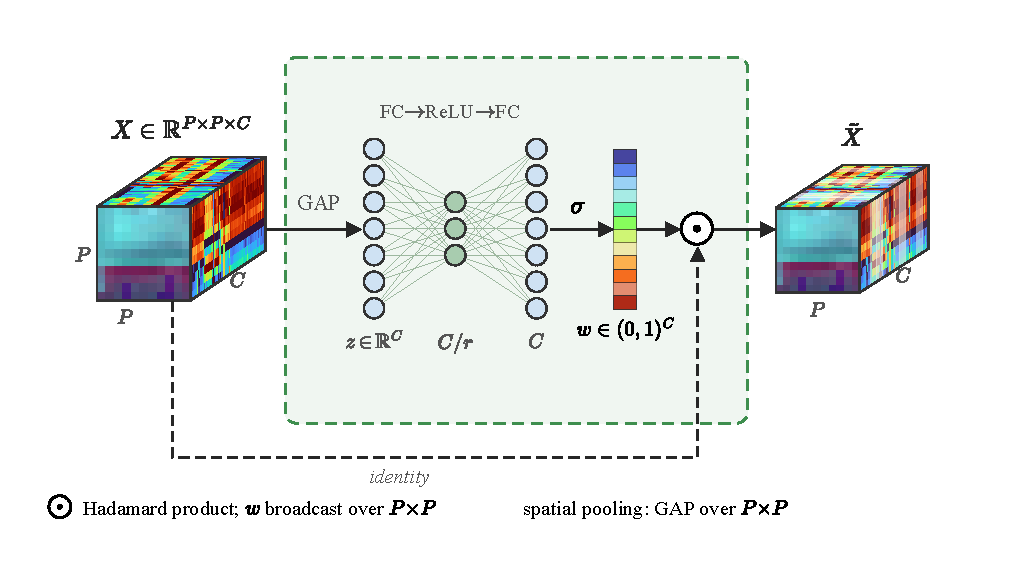
\includegraphics[width=0.32\textwidth]{figures/architecture/fig_sbam.pdf} &
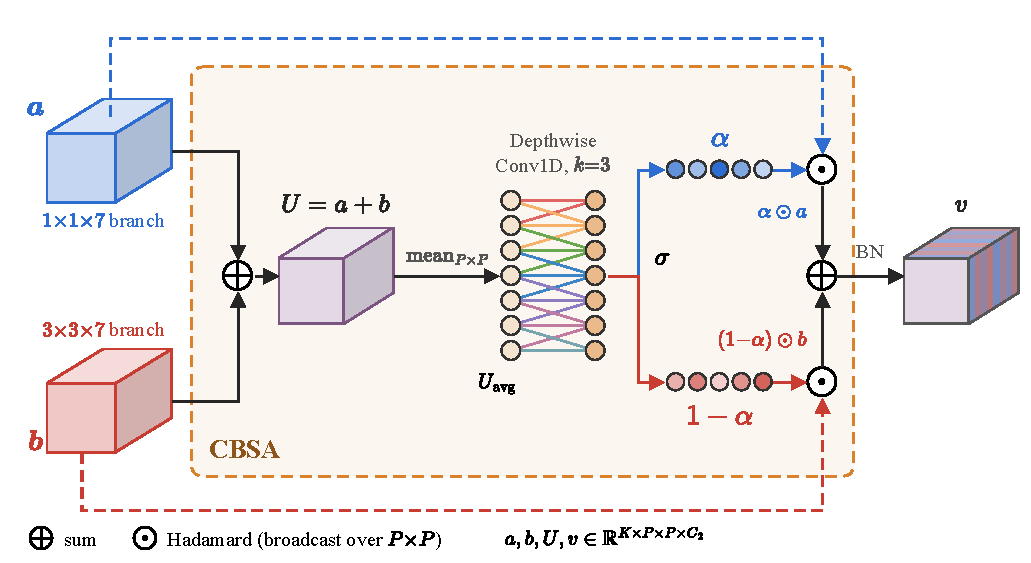
\includegraphics[width=0.32\textwidth]{figures/architecture/fig_cbsa.pdf} &
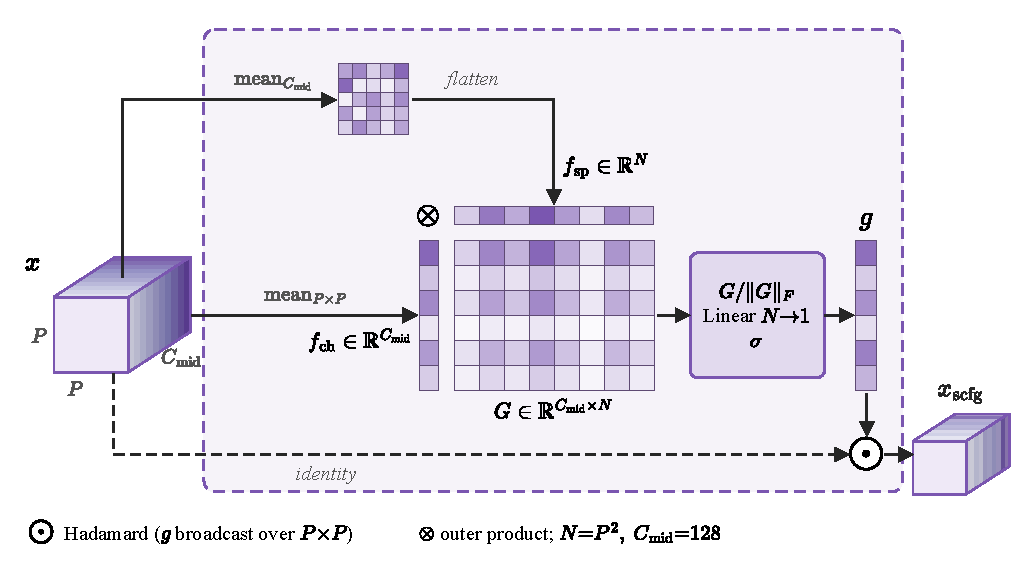
\includegraphics[width=0.32\textwidth]{figures/architecture/fig_scfg.pdf} \\
\footnotesize (a) SBAM & \footnotesize (b) CBSA & \footnotesize (c) SCFG \\
\end{tabular}
\caption{Detailed architectural topologies of the three proposed algorithmic modules: (a) Spectral Band Attention Module (SBAM) dynamically attenuating noisy atmospheric absorption bands on raw input cubes, (b) Complementary Branch Spectral Attention (CBSA) enforcing orthogonal specialization between dual 3D convolutional streams, and (c) Second-Order Covariance Fusion Gate (SCFG) capturing localized spatial-channel co-activation statistics.}
\label{fig:proposed_modules}
\Description{Architectural schematics of SBAM, CBSA, and SCFG modules.}
\end{figure*}

Hyperspectral sensors capture hundreds of contiguous spectral bands, but atmospheric water vapor absorption bands (such as those around 1.4 $\mu$m and 1.9 $\mu$m) and low signal-to-noise ratios at spectral boundaries corrupt raw reflectance signatures. Conventional deep learning architectures apply convolutional kernels indiscriminately across all raw bands, permitting noisy band responses to propagate into deep feature representations. While the Squeeze-and-Excitation Network (SENet) \cite{hu2018squeeze} and Convolutional Block Attention Module (CBAM) \cite{woo2018cbam} introduced channel and spatial attention, they operate strictly on deep latent feature maps following multiple convolutional stages. Unlike reinforcement learning band selection policies \cite{mou2022deep} or connected grouping heuristics \cite{guo2022feature} that require expensive outer optimization loops, SBAM embeds direct channel gating into the end-to-end differentiable graph.

To eliminate noise at the earliest computational stage, as illustrated in Fig.~\ref{fig:proposed_modules}(a), SBAM performs adaptive channel recalibration directly on raw spectral bands before any convolutional feature extraction. Given the input volumetric patch $X \in \mathbb{R}^{B \times 1 \times P \times P \times C}$, SBAM first compresses the spatial dimensions $P \times P$ via adaptive 3D average pooling to extract a global spectral descriptor $z \in \mathbb{R}^{B \times C}$:
\begin{equation}
\label{eq:sbam_pool}
z_c = \frac{1}{P^2} \sum_{u=1}^P \sum_{v=1}^P X(b, 1, u, v, c), \quad c \in \{1, 2, \dots, C\}
\end{equation}
To model inter-band dependencies while preserving low parameter complexity, the summary vector $z$ is routed through a multi-layer perceptron (MLP) bottleneck consisting of two linear projections with a dimensionality reduction ratio $r=8$:
\begin{equation}
\label{eq:sbam_fc}
w = \sigma\left(W_2 \cdot \delta(W_1 z + b_1) + b_2\right)
\end{equation}
where $W_1 \in \mathbb{R}^{C_{\text{mid}} \times C}$, $b_1 \in \mathbb{R}^{C_{\text{mid}}}$, $W_2 \in \mathbb{R}^{C \times C_{\text{mid}}}$, and $b_2 \in \mathbb{R}^{C}$. The bottleneck channel capacity is defined as $C_{\text{mid}} = \max(\lfloor C / r \rfloor, 8)$ to prevent over-compression on datasets with fewer spectral channels. Here, $\delta(\cdot)$ denotes the rectified linear unit (ReLU) activation, and $\sigma(\cdot)$ is the standard sigmoid gating function, yielding normalized band importance weights $w \in (0, 1)^{B \times C}$.

Finally, the input tensor $X$ is recalibrated via channel-wise broadcast multiplication:
\begin{equation}
\label{eq:sbam_recal}
\tilde{X} = X \odot \mathcal{E}(w), \quad \tilde{X} \in \mathbb{R}^{B \times 1 \times P \times P \times C}
\end{equation}
where $\mathcal{E}(w) \in \mathbb{R}^{B \times 1 \times 1 \times 1 \times C}$ denotes the broadcast expansion of $w$ across spatial dimensions, and $\odot$ represents element-wise Hadamard multiplication. By dynamically suppressing uninformative or corrupted spectral bands before convolution, SBAM shields downstream representation learning from atmospheric noise propagation.

\subsection{Complementary Branch Spectral Attention (CBSA)}
\label{subsec:cbsa}
Following SBAM recalibration, the refined tensor $\tilde{X}$ enters a dual-stream 3D convolutional module designed to capture multi-scale spectral and spatial structures concurrently:
\begin{equation}
\label{eq:cbsa_a}
a = \text{ReLU}\left(\text{BN}\left(\text{Conv3D}_{(1 \times 1 \times 7)}(\tilde{X})\right)\right) \in \mathbb{R}^{B \times K \times P \times P \times C_2}
\end{equation}
\begin{equation}
\label{eq:cbsa_b}
b = \text{ReLU}\left(\text{BN}\left(\text{Conv3D}_{(3 \times 3 \times 7)}(\tilde{X})\right)\right) \in \mathbb{R}^{B \times K \times P \times P \times C_2}
\end{equation}
where $K = 16$ denotes intermediate feature channels, and both 3D convolutions employ a spectral stride of 2, reducing the spectral dimension to $C_2 = \lfloor (C - 7) / 2 \rfloor + 1$. Branch $a$ uses a $1 \times 1 \times 7$ kernel focusing strictly on pure spectral inter-band transitions without spatial expansion. Branch $b$ applies a $3 \times 3 \times 7$ kernel with spatial padding $(1, 1, 0)$ to capture joint spatial-spectral context.

In multi-branch architectures such as A2S2K-ResNet \cite{roy2020attention}, Double-Branch networks \cite{li2020double}, and CSCANet \cite{wang2023cscanet}, parallel streams are combined either by direct summation or by computing a single shared squeeze-and-excitation attention gate. However, assigning an identical gating scalar to both streams causes them to learn co-dependent, redundant feature representations, negating the benefit of multi-scale branching.

To enforce orthogonal feature specialization, CBSA introduces a complementary gating mechanism. First, spatial context is aggregated across the fused representations $U = a + b$:
\begin{equation}
\label{eq:cbsa_u}
U_{\text{avg}} = \frac{1}{P^2} \sum_{u=1}^P \sum_{v=1}^P (a + b)[:, :, u, v, :] \in \mathbb{R}^{B \times K \times C_2}
\end{equation}
Next, a lightweight depthwise 1D convolution with kernel size $k_s = 3$ (grouped across $K$ channels, requiring only $K \times k_s = 48$ trainable parameters) models localized cross-band interactions:
\begin{equation}
\label{eq:cbsa_alpha}
\alpha = \sigma\left(\text{Conv1D}_{k_s}(U_{\text{avg}})\right) \in \mathbb{R}^{B \times K \times C_2}
\end{equation}
As depicted in Fig.~\ref{fig:proposed_modules}(b), expanding $\alpha$ to $\mathbb{R}^{B \times K \times 1 \times 1 \times C_2}$, the two branches are fused via complementary convex combination followed by 3D batch normalization:
\begin{equation}
\label{eq:cbsa_fuse}
v = \text{BN}\left(\alpha \odot a + (1 - \alpha) \odot b\right) \in \mathbb{R}^{B \times K \times P \times P \times C_2}
\end{equation}
Because the gating coefficients strictly satisfy $\alpha + (1 - \alpha) \equiv 1$ for every channel and band, CBSA forces competitive resource allocation between the streams. When spectral fidelity demands sharp discrimination, $\alpha \to 1$ promotes the pure spectral branch $a$ while suppressing spatial blurring from branch $b$. Conversely, in homogeneous spatial regions where neighborhood context dominates, $\alpha \to 0$ elevates branch $b$.

The fused representation $v$ is deepened through two consecutive 3D residual blocks equipped with 3D Efficient Channel Attention (ECA-3D) \cite{wang2020eca}:
\begin{equation}
\label{eq:spec_res}
v = \mathcal{R}_{\text{spec}}^{(2)}\left(\mathcal{R}_{\text{spec}}^{(1)}(v)\right) \in \mathbb{R}^{B \times K \times P \times P \times C_2}
\end{equation}
where each spectral residual block utilizes $1 \times 1 \times 7$ 3D convolutions with padding $(0, 0, 3)$ to preserve spatial-spectral dimensions while deepening feature abstraction.

\subsection{Second-Order Covariance Fusion Gate (SCFG)}
\label{subsec:scfg}
To transition from spectral-dominant processing to spatial context extraction, the spectral dimension $C_2$ is collapsed using adaptive 3D average pooling:
\begin{equation}
\label{eq:scfg_pool}
v_{\text{pool}} = \text{AdaptiveAvgPool3D}_{(P, P, 1)}(v) \in \mathbb{R}^{B \times K \times P \times P \times 1}
\end{equation}
A $1 \times 1 \times 1$ 3D convolution expands the channel dimension from $K=16$ to $C_{\text{mid}} = 128$:
\begin{equation}
\label{eq:scfg_expand}
v_{\text{exp}} = \text{ReLU}\left(\text{BN}\left(\text{Conv3D}_{(1 \times 1 \times 1)}(v_{\text{pool}})\right)\right) \in \mathbb{R}^{B \times C_{\text{mid}} \times P \times P \times 1}
\end{equation}
Squeezing the singleton spectral dimension yields the 2D spatial feature map $x \in \mathbb{R}^{B \times C_{\text{mid}} \times P \times P}$.

Standard spatial attention mechanisms and global pooling operators compute only first-order spatial means $\mu_c = \frac{1}{HW}\sum_{i} x_{c, i}$, discarding spatial co-activation structures. In heterogeneous land covers, specific semantic channels correlate with distinct spatial locations (e.g., edges versus interior textures). SCFG captures these second-order correlations through bilinear outer-product covariance modeling \cite{lin2015bilinear}.

Let $N = P \times P$ denote the total number of spatial pixels in the patch. We derive the global channel descriptor $f_{\text{ch}} \in \mathbb{R}^{B \times C_{\text{mid}}}$ and spatial position descriptor $f_{\text{sp}} \in \mathbb{R}^{B \times N}$:
\begin{equation}
\label{eq:scfg_descriptors}
f_{\text{ch}}(b, c) = \frac{1}{N} \sum_{n=1}^N x(b, c, n), \quad f_{\text{sp}}(b, n) = \frac{1}{C_{\text{mid}}} \sum_{c=1}^{C_{\text{mid}}} x(b, c, n)
\end{equation}
The second-order spatial-channel covariance interaction matrix $G \in \mathbb{R}^{B \times C_{\text{mid}} \times N}$ is computed via batch outer product:
\begin{equation}
\label{eq:scfg_g}
G = f_{\text{ch}} \otimes f_{\text{sp}} = f_{\text{ch}} f_{\text{sp}}^T, \quad G(b, c, n) = f_{\text{ch}}(b, c) \cdot f_{\text{sp}}(b, n)
\end{equation}
Each matrix entry $G(b, c, n)$ measures the bilinear co-occurrence strength between channel $c$ and spatial coordinate $n$, extending second-order covariance principles from fine-grained recognition \cite{lin2015bilinear, gao2019global} and HSI covariance modeling \cite{fang2018new, he2019feature, xue2021attention, zheng2021hyperspectral} into an efficient spatial-channel gating operator without requiring iterative matrix square-root decompositions \cite{li2018towards}.

To guarantee numerical stability and invariant gradient scaling across varied patch dynamics, $G$ is normalized by its Frobenius norm:
\begin{equation}
\label{eq:scfg_frob}
\tilde{G} = \frac{G}{\|G\|_F + \epsilon} = \frac{G}{\sqrt{\sum_{c=1}^{C_{\text{mid}}} \sum_{n=1}^N G(b, c, n)^2} + \epsilon}
\end{equation}
where $\epsilon = 10^{-8}$. A learnable linear projection $W_G \in \mathbb{R}^{1 \times N}$ compresses the spatial interaction dimension of $\tilde{G}$ into a channel-wise modulation gate:
\begin{equation}
\label{eq:scfg_gate}
g = \sigma\left(W_G \tilde{G}\right) \in \mathbb{R}^{B \times C_{\text{mid}}}
\end{equation}
The recalibrated feature map is obtained by element-wise modulation:
\begin{equation}
\label{eq:scfg_mod}
x_{\text{scfg}} = x \odot g
\end{equation}
where $g$ is broadcast across the spatial grid $P \times P$.

To process spatial context, $x_{\text{scfg}}$ is reshaped by permuting spatial and channel axes into a 3D volumetric tensor $v_{\text{spat}} \in \mathbb{R}^{B \times 1 \times P \times P \times C_{\text{mid}}}$, treating the 128 channels as the spectral/depth dimension for 3D convolution. A spatial entry convolution $\text{Conv3D}_{(3 \times 3 \times 128)}$ projects the tensor to $K=16$ feature maps:
\begin{equation}
\label{eq:spat_entry}
s = \text{ReLU}\left(\text{BN}\left(\text{Conv3D}_{(3 \times 3 \times 128)}(v_{\text{spat}})\right)\right) \in \mathbb{R}^{B \times K \times P \times P \times 1}
\end{equation}
The tensor is processed through two cascaded spatial 3D residual blocks with $3 \times 3 \times 1$ convolutions and ECA-3D attention:
\begin{equation}
\label{eq:spat_res}
s_{\text{out}} = \mathcal{R}_{\text{spat}}^{(2)}\left(\mathcal{R}_{\text{spat}}^{(1)}(s)\right) \in \mathbb{R}^{B \times K \times P \times P \times 1}
\end{equation}
Finally, 3D adaptive average pooling collapses spatial dimensions to extract a $K$-dimensional latent representation $z \in \mathbb{R}^{B \times K}$:
\begin{equation}
\label{eq:global_pool}
z = \text{AdaptiveAvgPool3D}_{(1,1,1)}(s_{\text{out}})
\end{equation}
The latent vector $z$ is subsequently projected to class logits $\hat{y} \in \mathbb{R}^{B \times C_{\text{cls}}}$ by a linear classification head:
\begin{equation}
\label{eq:fc_out}
\hat{y} = W_{\text{fc}} z + b_{\text{fc}}
\end{equation}

\subsection{Minority-Aware Hybrid Loss Formulation}
\label{subsec:loss}
Hyperspectral benchmark datasets exhibit severe class imbalance. For example, in Indian Pines, dominant classes such as Soybean-mintill contain 2,468 labeled pixels, whereas rare categories such as Oats and Grass-pasture-mowed contain only 20 and 28 samples, respectively. Standard cross-entropy loss gradients become heavily dominated by prevalent categories, causing catastrophic decision boundary collapse on minority land covers.

To establish wide, robust decision boundaries while prioritizing under-represented categories, SGSCF-Net is trained with a hybrid objective combining margin-scheduled Spread Loss \cite{sabour2018matrix} and inverse-frequency class-weighted Focal Loss \cite{lin2017focal}, drawing upon margin optimization and sample-effective regularization principles \cite{cui2019class, cao2019learning, haut2021generative}.

\subsubsection{Dynamic Margin-Scheduled Spread Loss}
Spread Loss directly penalizes predictions where non-target class activations fall within a specified margin $m$ of the true class logit:
\begin{equation}
\label{eq:spread_loss}
\mathcal{L}_{\text{Spread}} = \frac{1}{B} \sum_{i=1}^B \sum_{j \neq y_i} \left(\max\left(0, m(r) - (a_{y_i} - a_j)\right)\right)^2
\end{equation}
where $a_k$ represents the output activation for class $k$, and $m(r)$ is a dynamic margin scheduled linearly according to the training progression ratio $r = \frac{t}{T_{\text{total}}} \in [0, 1]$:
\begin{equation}
\label{eq:margin_sched}
m(r) = m_{\min} + (m_{\max} - m_{\min}) \cdot r
\end{equation}
with $m_{\min} = 0.2$ and $m_{\max} = 0.9$. In early epochs ($r \to 0$), a relaxed margin $m=0.2$ prevents over-penalizing uncalibrated initial weights; in late epochs ($r \to 1$), the margin expands to $0.9$, compelling the model to enforce wide decision boundaries between competing categories.

\subsubsection{Inverse-Frequency Class-Weighted Focal Loss}
To prevent dominant majority classes from overwhelming the gradient signal and to focus optimization on hard samples, we integrate Focal Loss:
\begin{equation}
\label{eq:focal_loss}
\mathcal{L}_{\text{Focal}} = -\frac{1}{B} \sum_{i=1}^B \alpha_{y_i} (1 - p_{t, i})^\gamma \log(p_{t, i})
\end{equation}
where $p_{t, i} = \frac{\exp(\hat{y}_{i, y_i})}{\sum_k \exp(\hat{y}_{i, k})}$ is the softmax probability of the ground-truth class, $\gamma = 2.0$ is the focusing parameter, and $\alpha_c$ is the normalized inverse-frequency weight for class $c \in \{1, \dots, C_{\text{cls}}\}$:
\begin{equation}
\label{eq:class_weights}
w_c = \frac{1}{N_c + \epsilon}, \quad \alpha_c = \frac{w_c}{\sum_{k=1}^{C_{\text{cls}}} w_k} \cdot C_{\text{cls}}
\end{equation}
where $N_c$ is the total count of training samples belonging to class $c$.

\subsubsection{Combined Optimization Objective}
The total end-to-end training loss is defined as:
\begin{equation}
\label{eq:total_loss}
\mathcal{L}_{\text{Total}} = 0.7 \mathcal{L}_{\text{Spread}} + 0.3 \mathcal{L}_{\text{Focal}}
\end{equation}
This hybrid objective balances margin spread across competing categories with hard-sample focal mining, ensuring balanced gradient contributions and preventing minority class collapse under extreme sample scarcity.

\section{Experiments and Comparative Analysis}
\label{sec:experiments}
This section presents an empirical evaluation of SGSCF-Net alongside eight standardized baseline models. We first describe the benchmark hyperspectral datasets and provide comprehensive category distributions. Next, we outline the experimental setup, comparative models, and evaluation metrics. Finally, we report quantitative comparisons on Indian Pines, examine computational latency, and analyze parameter efficiency.

\subsection{Dataset Description}
\label{subsec:datasets}
To evaluate model performance across heterogeneous spatial resolutions, sensor configurations, and land-cover categories, experiments are conducted on three standard benchmark datasets: Indian Pines, Pavia University, and Salinas Valley. In all experiments, labeled samples are partitioned into training, validation, and testing sets following a standard 10\%, 10\%, and 80\% stratified split per class. A structured summary of sensor properties, spatial dimensions, spectral channels, and sample allocations for each benchmark is provided in Table~\ref{tab:dataset_summary}. For each benchmark, the corresponding subsection below first describes the acquisition protocol and land-cover composition, and then reports the per-class ground-truth colour palette together with the stratified sample allocation (Tables~\ref{tab:cat_ip}, \ref{tab:cat_pu}, and \ref{tab:cat_sv}). These palettes are retained consistently throughout the classification maps rendered for each dataset in the subsequent sections.

\begin{table*}[t]
\centering
\footnotesize
\caption{Benchmark Hyperspectral Dataset Characteristics and Sample Allocations (10\% Train / 10\% Val / 80\% Test Split).}
\label{tab:dataset_summary}
\begin{tabular*}{\textwidth}{@{\extracolsep{\fill}}lcccccccc}
\toprule
\textbf{Dataset} & \textbf{Sensor} & \textbf{Range ($\mu$m)} & \textbf{Bands} & \textbf{Spatial Size} & \textbf{Res. (m)} & \textbf{Classes} & \textbf{Labeled Pixels} & \textbf{Train / Val / Test} \\
\midrule
Indian Pines & AVIRIS & 0.40--2.50 & 200 & $145 \times 145$ & 20.0 & 16 & 10,249 & 1,025 / 1,025 / 8,199 \\
Pavia University & ROSIS-03 & 0.43--0.86 & 103 & $610 \times 340$ & 1.3 & 9 & 42,776 & 4,277 / 4,277 / 34,222 \\
Salinas Valley & AVIRIS & 0.40--2.50 & 204 & $512 \times 217$ & 3.7 & 16 & 54,129 & 5,413 / 5,413 / 43,303 \\
\bottomrule
\end{tabular*}
\end{table*}

\subsubsection{Indian Pines}
The Indian Pines dataset was gathered in 1992 by the Airborne Visible/Infrared Imaging Spectrometer (AVIRIS) sensor \cite{green1998imaging} over an agricultural test site in Northwest Indiana. The spatial scene measures $145 \times 145$ pixels with a moderate spatial resolution of 20 m per pixel. The sensor records 224 contiguous spectral bands spanning the 0.4--2.5 $\mu$m wavelength range. Following standard experimental protocol, 20 water-absorption and noise-corrupted bands (bands 104--108, 150--163, and 220) are excluded, leaving 200 clean spectral channels. The ground truth contains 16 land-cover categories encompassing two-thirds agricultural crops (e.g., corn, soybeans, wheat) and one-third natural vegetation (e.g., woods, grass). A total of 10,249 pixels are labeled. Indian Pines presents acute class imbalance: dominant categories such as Soybean-mintill comprise 2,468 samples, whereas minority classes such as Oats and Grass-pasture-mowed contain only 20 and 28 samples, respectively. The per-class ground-truth colour palette and stratified sample allocation are listed in Table~\ref{tab:cat_ip}.

\begin{table}[htbp]
\centering
\footnotesize
\caption{Category Information of the Indian Pines Dataset. Train/Val/Test counts follow a stratified 10\%/10\%/80\% split per class.}
\label{tab:cat_ip}
\begin{tabular}{clcccc}
\toprule
\textbf{ID} & \textbf{Colour \quad Class Name} & \textbf{Train} & \textbf{Val} & \textbf{Test} & \textbf{Total} \\
\midrule
1  & \clrsw{ipA}~Alfalfa                        & 5    & 5    & 36    & 46 \\
2  & \clrsw{ipB}~Corn-notill                    & 143  & 143  & 1,142 & 1,428 \\
3  & \clrsw{ipC}~Corn-mintill                   & 83   & 83   & 664   & 830 \\
4  & \clrsw{ipD}~Corn                           & 24   & 24   & 189   & 237 \\
5  & \clrsw{ipE}~Grass-pasture                  & 48   & 48   & 387   & 483 \\
6  & \clrsw{ipF}~Grass-trees                    & 73   & 73   & 584   & 730 \\
7  & \clrsw{ipG}~Grass-pasture-mowed            & 3    & 3    & 22    & 28 \\
8  & \clrsw{ipH}~Hay-windrowed                  & 48   & 48   & 382   & 478 \\
9  & \clrsw{ipI}~Oats                           & 2    & 2    & 16    & 20 \\
10 & \clrsw{ipJ}~Soybean-notill                 & 97   & 97   & 778   & 972 \\
11 & \clrsw{ipK}~Soybean-mintill                & 246  & 246  & 1,963 & 2,455 \\
12 & \clrsw{ipL}~Soybean-clean                  & 59   & 59   & 475   & 593 \\
13 & \clrsw{ipM}~Wheat                          & 21   & 21   & 163   & 205 \\
14 & \clrsw{ipN}~Woods                          & 127  & 127  & 1,011 & 1,265 \\
15 & \clrsw{ipO}~Buildings-Grass-Trees-Drives   & 39   & 39   & 308   & 386 \\
16 & \clrsw{ipP}~Stone-Steel-Towers             & 9    & 9    & 75    & 93 \\
\midrule
   & \textbf{Total}                              & \textbf{1,025} & \textbf{1,025} & \textbf{8,199} & \textbf{10,249} \\
\bottomrule
\end{tabular}
\end{table}

\subsubsection{Pavia University}
The Pavia University dataset was acquired by the Reflective Optics System Imaging Spectrometer (ROSIS-03) sensor during an aerial flight campaign over Pavia, Northern Italy \cite{fauvel2008spectral}. The image dimensions are $610 \times 340$ pixels with a fine spatial resolution of 1.3 m per pixel. The sensor covers the spectral range from 430 to 860 nm across 115 bands. After discarding 12 heavily corrupted atmospheric noise bands, 103 calibrated spectral channels are retained. The ground-truth reference map contains nine urban land-cover classes, including asphalt roads, meadows, gravel, trees, painted metal sheets, bare soil, bitumen, self-blocking bricks, and shadows. The scene contains 42,776 labeled pixels, characterized by complex geometric boundaries and high intra-class spatial variance. The per-class ground-truth colour palette and stratified sample allocation are listed in Table~\ref{tab:cat_pu}.

\begin{table}[htbp]
\centering
\footnotesize
\caption{Category Information of the Pavia University Dataset. Train/Val/Test counts follow a stratified 10\%/10\%/80\% split per class.}
\label{tab:cat_pu}
\begin{tabular}{clcccc}
\toprule
\textbf{ID} & \textbf{Colour \quad Class Name} & \textbf{Train} & \textbf{Val} & \textbf{Test} & \textbf{Total} \\
\midrule
1 & \clrsw{ipA}~Asphalt              & 663   & 663   & 5,305  & 6,631 \\
2 & \clrsw{ipB}~Meadows              & 1,865 & 1,865 & 14,919 & 18,649 \\
3 & \clrsw{ipC}~Gravel               & 210   & 210   & 1,679  & 2,099 \\
4 & \clrsw{ipD}~Trees                & 306   & 306   & 2,452  & 3,064 \\
5 & \clrsw{ipE}~Painted metal sheets & 134   & 134   & 1,077  & 1,345 \\
6 & \clrsw{ipF}~Bare Soil            & 503   & 503   & 4,023  & 5,029 \\
7 & \clrsw{ipG}~Bitumen              & 133   & 133   & 1,064  & 1,330 \\
8 & \clrsw{ipH}~Self-Blocking Bricks & 368   & 368   & 2,946  & 3,682 \\
9 & \clrsw{ipI}~Shadows              & 95    & 95    & 757    & 947 \\
\midrule
  & \textbf{Total}                   & \textbf{4,277} & \textbf{4,277} & \textbf{34,222} & \textbf{42,776} \\
\bottomrule
\end{tabular}
\end{table}

\subsubsection{Salinas Valley}
The Salinas Valley dataset was captured by the AVIRIS sensor \cite{green1998imaging} over the fertile Salinas Valley agricultural region in California. The dataset covers $512 \times 217$ pixels with a spatial resolution of 3.7 m per pixel. The spectrometer records 224 bands across 0.4--2.5 $\mu$m. Discarding 20 water-vapor absorption bands (bands 108--112, 154--167, and 224) yields 204 usable spectral channels. The ground truth comprises 16 agricultural land-cover classes, including multiple cultivars of lettuce at distinct growth stages (e.g., 4-week, 5-week, 6-week, and 7-week Romaine), broccoli, celery, grapes, and vineyard fields. A total of 54,129 pixels are labeled. The per-class ground-truth colour palette and stratified sample allocation are listed in Table~\ref{tab:cat_sv}.

\begin{table}[htbp]
\centering
\footnotesize
\caption{Category Information of the Salinas Valley Dataset. Train/Val/Test counts follow a stratified 10\%/10\%/80\% split per class.}
\label{tab:cat_sv}
\begin{tabular}{clcccc}
\toprule
\textbf{ID} & \textbf{Colour \quad Class Name} & \textbf{Train} & \textbf{Val} & \textbf{Test} & \textbf{Total} \\
\midrule
1  & \clrsw{ipA}~Brocoli\_green\_weeds\_1        & 201   & 201   & 1,607 & 2,009 \\
2  & \clrsw{ipB}~Brocoli\_green\_weeds\_2        & 373   & 373   & 2,980 & 3,726 \\
3  & \clrsw{ipC}~Fallow                           & 198   & 198   & 1,580 & 1,976 \\
4  & \clrsw{ipD}~Fallow\_rough\_plow              & 139   & 139   & 1,116 & 1,394 \\
5  & \clrsw{ipE}~Fallow\_smooth                   & 268   & 268   & 2,142 & 2,678 \\
6  & \clrsw{ipF}~Stubble                          & 396   & 396   & 3,167 & 3,959 \\
7  & \clrsw{ipG}~Celery                           & 358   & 358   & 2,863 & 3,579 \\
8  & \clrsw{ipH}~Grapes\_untrained                & 1,127 & 1,127 & 9,017 & 11,271 \\
9  & \clrsw{ipI}~Soil\_vinyard\_develop           & 620   & 620   & 4,963 & 6,203 \\
10 & \clrsw{ipJ}~Corn\_senesced\_green\_weeds    & 328   & 328   & 2,622 & 3,278 \\
11 & \clrsw{ipK}~Lettuce\_romaine\_4wk            & 107   & 107   & 854   & 1,068 \\
12 & \clrsw{ipL}~Lettuce\_romaine\_5wk            & 193   & 193   & 1,541 & 1,927 \\
13 & \clrsw{ipM}~Lettuce\_romaine\_6wk            & 92    & 92    & 732   & 916 \\
14 & \clrsw{ipN}~Lettuce\_romaine\_7wk            & 107   & 107   & 856   & 1,070 \\
15 & \clrsw{ipO}~Vinyard\_untrained               & 727   & 727   & 5,814 & 7,268 \\
16 & \clrsw{ipP}~Vinyard\_vertical\_trellis       & 181   & 181   & 1,445 & 1,807 \\
\midrule
   & \textbf{Total}                                & \textbf{5,413} & \textbf{5,413} & \textbf{43,303} & \textbf{54,129} \\
\bottomrule
\end{tabular}
\end{table}

\subsection{Implementation Details}
\label{subsec:implementation}

\subsubsection{Compared Methods}
SGSCF-Net is benchmarked against eight representative baselines across four architectural paradigms, evaluated using their official open-source implementations: 3D residual CNNs (SSRN~\cite{zhong2017spectral}\footnote{\url{https://github.com/zilongzhong/SSRN}}, A2S2K-ResNet~\cite{roy2020attention}\footnote{\url{https://github.com/suvojit-0x55aa/A2S2K-ResNet}}), decoupled attention networks (SSAN~\cite{sun2019spectral}\footnote{\url{https://github.com/EtPan/SSAN}}), vision transformers (standard ViT~\cite{dosovitskiy2020image}\footnote{\url{https://github.com/google-research/vision_transformer}}, tokenized HSI-SSFTT~\cite{sun2022spectral}\footnote{\url{https://github.com/zgr6010/HSI_SSFTT}}, and rotary-embedded HyperRoPE-HiT~\cite{khan2025hyperrope}\footnote{\url{https://github.com/zirakkk/hyperrope-sst}}), and hybrid/capsule networks (CRV-MHDL~\cite{alalimi2022compression}\footnote{\url{https://github.com/DalalAL-Alimi/CRV}} and EM-routed DMC~\cite{wang2021deep}\footnote{\url{https://github.com/DeepMatrixCapsules/DeepMatrixCapsules}}).

\subsubsection{Evaluation Metrics}
Model performance is quantified across three standard objective metrics: Overall Accuracy (OA, \%), Average Accuracy (AA, \%), and Cohen's Kappa coefficient ($\kappa \times 100$). OA measures the proportion of correctly classified test samples over total test samples:
\begin{equation}
\label{eq:oa}
\text{OA} = \frac{\sum_{i=1}^{C_{\text{cls}}} M_{ii}}{\sum_{i=1}^{C_{\text{cls}}} \sum_{j=1}^{C_{\text{cls}}} M_{ij}} \times 100\%
\end{equation}
where $M \in \mathbb{R}^{C_{\text{cls}} \times C_{\text{cls}}}$ denotes the classification confusion matrix, and $M_{ij}$ indicates the number of samples belonging to ground-truth class $i$ classified into class $j$. AA computes the unweighted arithmetic mean of per-class accuracies:
\begin{equation}
\label{eq:aa}
\text{AA} = \frac{1}{C_{\text{cls}}} \sum_{i=1}^{C_{\text{cls}}} \frac{M_{ii}}{\sum_{j=1}^{C_{\text{cls}}} M_{ij}} \times 100\%
\end{equation}
AA directly reflects classification robustness across skewed class distributions. Cohen's Kappa ($\kappa$) quantifies statistical agreement adjusted for chance:
\begin{equation}
\label{eq:kappa}
\kappa = \frac{P_o - P_e}{1 - P_e} \times 100
\end{equation}
where $P_o = \text{OA} / 100$, and $P_e = \frac{\sum_{i=1}^{C_{\text{cls}}} (\sum_{j} M_{ij})(\sum_{j} M_{ji})}{(\sum_{i,j} M_{ij})^2}$. Additionally, wall-clock training duration (minutes) is tracked to evaluate computational efficiency.

\subsubsection{Experimental Configuration}
All models are executed within a unified PyTorch framework accelerated on an NVIDIA GPU environment. For SGSCF-Net, model weights are optimized via the Adam optimizer with an initial learning rate of $\eta = 5 \times 10^{-4}$, scheduled through a Cosine Annealing decay down to $\eta_{\min} = 10^{-6}$ over 200 epochs. Gradients are clipped at a maximum $\ell_2$-norm threshold of 5.0 to ensure numerical stability. The input spatial patch size is fixed at $11 \times 11$, and the batch size is set to 32. For baseline models (SSRN, A2S2K-ResNet, SSAN, ViT, HSI-SSFTT, HyperRoPE-HiT, CRV-MHDL, and DMC), standard architectures and recommended hyperparameters are strictly adhered to under identical 10\%/10\%/80\% data splits to ensure fair and reproducible benchmarking.

\subsection{Comparative Study on Indian Pines}
\label{subsec:comparative_study}
Table~\ref{tab:perclass_ip} presents the quantitative per-class, overall, and average classification results across all nine models evaluated on the Indian Pines test set.

As demonstrated in Table~\ref{tab:perclass_ip}, SGSCF-Net achieves 98.05\% Overall Accuracy, 94.82\% Average Accuracy, and 97.78 Kappa on Indian Pines. Although SSRN posts a marginally higher Overall Accuracy (98.52\%), its Average Accuracy collapses to 79.99\% because it fails completely on the three smallest classes---Alfalfa, Grass-pasture-mowed, and Oats---each scoring 0.00\%. SGSCF-Net instead delivers the highest Average Accuracy of all nine models (94.82\%), narrowly ahead of A2S2K-ResNet (94.41\%) and HSI-SSFTT (94.29\%), confirming that the minority-aware hybrid objective protects rare land-cover boundaries rather than trading them for majority-class gains. The margin over the standard Vision Transformer (ViT, 90.33\% OA) reaches +7.72\% OA, and SGSCF-Net remains robust where the capsule and compression baselines degrade sharply (DMC 82.55\% OA, CRV-MHDL 67.20\% OA).

Granular per-class results, reported in Table~\ref{tab:perclass_ip}, further confirm this robustness. Dominant agricultural categories such as Hay-windrowed (478 pixels) and Corn (237 pixels) saturate at 100.00\% accuracy, while the Soybean cluster---often confused by baseline methods---retains 98.84\% (Soybean-notill), 98.42\% (Soybean-mintill), and 91.85\% (Soybean-clean). Among the three extreme-minority categories (Alfalfa, Grass-pasture-mowed, and Oats with only 46, 28, and 20 labelled pixels respectively), SGSCF-Net preserves 95.00\%, 95.24\%, and 54.17\% accuracy. The Oats drop reflects the hard information floor imposed by only two training patches per class; nonetheless, the minority-aware hybrid objective ($\mathcal{L} = 0.7\mathcal{L}_{\text{Spread}} + 0.3\mathcal{L}_{\text{Focal}}$) prevents the complete decision-boundary collapse observed in SSAN (which drops to 64.19\% OA because its unweighted cross-entropy gradient is dominated by Soybean-mintill).

\begin{table*}[tbp]
\centering
\scriptsize
\setlength{\tabcolsep}{3.5pt}
\caption{Per-Class Classification Accuracy (\%) of SGSCF-Net and Eight Baseline Models on the Indian Pines Test Set (10\% Train / 10\% Val / 80\% Test, Patch 11$\times$11, Batch 32, 200 Epochs). Overall Accuracy (OA), Average Accuracy (AA), Kappa ($\kappa \times 100$), and training time are reported in the final rows. Best OA/AA/$\kappa$ in bold.}
\label{tab:perclass_ip}
\begin{tabular}{p{3.0cm}ccccccccc}
\toprule
\textbf{Class} & \textbf{SSRN} & \textbf{HyperRoPE} & \textbf{A2S2K} & \textbf{SSFTT} & \textbf{DMC} & \textbf{ViT} & \textbf{CRV} & \textbf{SSAN} & \textbf{Ours} \\
\midrule
Alfalfa                      & 0.00 & 94.44 & 94.44 & 83.78 & 2.70 & 70.27 & 10.81 & 71.88 & 95.00 \\
Corn-notill                  & 96.44 & 93.87 & 98.50 & 95.36 & 77.41 & 82.14 & 47.64 & 65.96 & 98.13 \\
Corn-mintill                 & 98.81 & 95.63 & 98.47 & 99.70 & 73.04 & 78.46 & 43.07 & 78.41 & 97.72 \\
Corn                         & 98.18 & 83.07 & 100.00 & 98.41 & 24.87 & 90.48 & 9.52 & 76.36 & 100.00 \\
Grass-pasture                & 97.17 & 89.66 & 97.96 & 99.22 & 90.96 & 90.18 & 85.01 & 84.10 & 99.74 \\
Grass-trees                  & 99.42 & 96.23 & 97.18 & 99.32 & 96.40 & 96.75 & 97.26 & 96.79 & 99.17 \\
Grass-pasture-mowed          & 0.00 & 90.91 & 100.00 & 100.00 & 0.00 & 95.45 & 9.09 & 60.00 & 95.24 \\
Hay-windrowed                & 95.89 & 100.00 & 99.48 & 100.00 & 99.74 & 99.48 & 84.29 & 98.20 & 100.00 \\
Oats                         & 0.00 & 25.00 & 50.00 & 43.75 & 0.00 & 68.75 & 18.75 & 14.29 & 54.17 \\
Soybean-notill               & 99.12 & 94.94 & 98.04 & 98.84 & 76.61 & 83.55 & 63.37 & 72.15 & 98.84 \\
Soybean-mintill              & 99.24 & 95.87 & 99.03 & 99.24 & 91.30 & 92.37 & 75.27 & 25.76 & 98.42 \\
Soybean-clean                & 99.28 & 83.37 & 94.29 & 96.63 & 47.16 & 89.26 & 39.79 & 52.16 & 91.85 \\
Wheat                        & 100.00 & 98.79 & 97.53 & 100.00 & 91.46 & 97.56 & 94.51 & 94.41 & 99.39 \\
Woods                        & 99.10 & 94.37 & 99.31 & 99.70 & 97.53 & 99.80 & 97.63 & 92.58 & 98.65 \\
Buildings-Grass-Trees-Drives & 100.00 & 93.83 & 96.19 & 100.00 & 80.52 & 95.45 & 39.29 & 82.80 & 99.00 \\
Stone-Steel-Towers           & 97.18 & 100.00 & 90.12 & 94.67 & 76.00 & 96.00 & 12.00 & 98.46 & 91.89 \\
\midrule
\textbf{OA}          & \textbf{98.52} & 94.07 & 98.11 & 98.45 & 82.55 & 90.33 & 67.20 & 64.19 & 98.05 \\
\textbf{AA}          & 79.99 & 89.37 & 94.41 & 94.29 & 64.11 & 89.12 & 51.71 & 72.77 & \textbf{94.82} \\
\textbf{Kappa ($\kappa\times100$)} & \textbf{98.31} & 93.24 & 97.85 & 98.23 & 79.89 & 88.95 & 62.22 & 59.79 & 97.78 \\
\bottomrule
\end{tabular}
\flushleft
\footnotesize{Baseline per-class accuracies are evaluated on the held-out 80\% test split from each model's standardized Indian Pines benchmark run. ``HyperRoPE'' denotes the HyperRoPE-HiT variant. SSRN attains the highest OA but collapses on the three extreme-minority classes (Alfalfa, Grass-pasture-mowed, Oats at 0.00\%), yielding the lowest AA among competitive models; SGSCF-Net attains the best Average Accuracy (94.82\%). DMC patches were zero-padded from 11$\times$11 to 13$\times$13 to satisfy capsule squash requirements.}
\end{table*}

Fig.~\ref{fig:indian_pines_maps} illustrates the qualitative classification maps generated by all evaluated models on the Indian Pines scene alongside the ground-truth reference map. Visual comparison reveals pronounced differences across architectural paradigms. The attention network SSAN (Fig.~\ref{fig:indian_pines_maps}(e)) suffers from severe spatial misclassification and extensive salt-and-pepper noise, misidentifying entire sections of Corn and Soybean parcels due to gradient starvation on smaller categories. Transformer-based models such as ViT (Fig.~\ref{fig:indian_pines_maps}(b)) and HyperRoPE-HiT (Fig.~\ref{fig:indian_pines_maps}(h)) resolve general thematic clusters but produce noticeable edge blurring and over-smoothed transitions along narrow field margins. The capsule network DMC (Fig.~\ref{fig:indian_pines_maps}(i)) and the compression-based CRV-MHDL (Fig.~\ref{fig:indian_pines_maps}(g)) degrade markedly on this imbalanced scene (82.55\% and 67.20\% OA), scattering misclassifications across the Corn and Soybean parcels and erasing the smallest categories. In contrast, the 3D convolutional and tokenizer models (SSRN, A2S2K-ResNet, HSI-SSFTT) reproduce cleaner regional coherence, aligning with regional contextual boundaries in diverse region CNNs \cite{zhang2018diverse}; yet SSRN, despite its high overall accuracy, blanks out the rare Alfalfa, Grass-pasture-mowed, and Oats parcels entirely. SGSCF-Net (Fig.~\ref{fig:indian_pines_maps}(j)) produces the most visually contiguous and balanced thematic map among the trained models: interior field parcels are exceptionally homogeneous, parcel borders remain sharply delineated, and noise-induced scattering is effectively suppressed. This confirms that the input-level SBAM filtering and complementary CBSA gating successfully isolate true reflectance boundaries from atmospheric noise.

\begin{figure*}[t]
\centering
\setlength{\tabcolsep}{2pt}
\begin{tabular}{ccccc}
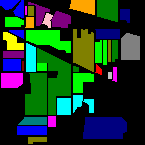
\includegraphics[width=0.19\textwidth]{figures/ip_gt.png} &
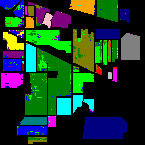
\includegraphics[width=0.19\textwidth]{figures/ip_vit.png} &
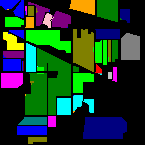
\includegraphics[width=0.19\textwidth]{figures/ip_ssftt.png} &
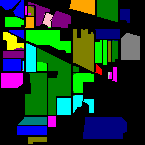
\includegraphics[width=0.19\textwidth]{figures/ip_ssrn.png} &
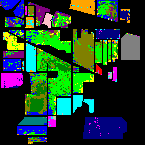
\includegraphics[width=0.19\textwidth]{figures/ip_ssan.png} \\
\footnotesize (a) Ground Truth &
\footnotesize (b) ViT \cite{dosovitskiy2020image} &
\footnotesize (c) HSI-SSFTT \cite{sun2022spectral} &
\footnotesize (d) SSRN \cite{zhong2017spectral} &
\footnotesize (e) SSAN \cite{sun2019spectral} \\[4pt]
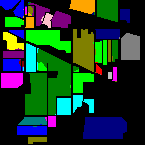
\includegraphics[width=0.19\textwidth]{figures/ip_a2s2k.png} &
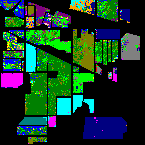
\includegraphics[width=0.19\textwidth]{figures/ip_crv.png} &
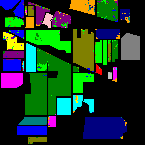
\includegraphics[width=0.19\textwidth]{figures/ip_hit.png} &
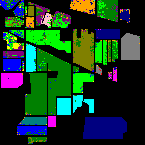
\includegraphics[width=0.19\textwidth]{figures/ip_dmc.png} &
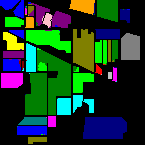
\includegraphics[width=0.19\textwidth]{figures/ip_sgscfnet.png} \\
\footnotesize (f) A2S2K-ResNet \cite{roy2020attention} &
\footnotesize (g) CRV-MHDL \cite{alalimi2022compression} &
\footnotesize (h) HyperRoPE-HiT \cite{khan2025hyperrope} &
\footnotesize (i) DMC \cite{wang2021deep} &
\footnotesize (j) SGSCF-Net (\textbf{Ours}) \\
\end{tabular}
\caption{Classification maps of different methods for the Indian Pines dataset under standardized 10\% training ratio. (a) Ground truth. (b) ViT (OA: 90.33\%). (c) HSI-SSFTT (OA: 98.45\%). (d) SSRN (OA: 98.52\%). (e) SSAN (OA: 64.19\%). (f) A2S2K-ResNet (OA: 98.11\%). (g) CRV-MHDL (OA: 67.20\%). (h) HyperRoPE-HiT (OA: 94.07\%). (i) DMC (OA: 82.55\%). (j) SGSCF-Net (Ours, OA: 98.05\%).}
\label{fig:indian_pines_maps}
\Description{Classification maps of the Indian Pines dataset comparing ground truth, eight baseline models, and SGSCF-Net.}
\end{figure*}

\subsection{Comparative Study on Pavia University}
\label{subsec:pavia_study}
The Pavia University benchmark evaluates model robustness on high-spatial-resolution (1.3-m) urban remote sensing imagery. Table~\ref{tab:perclass_pu} reports the per-class, overall, and average classification performance across all nine evaluated architectures under standardized 10\% training, 10\% validation, and 80\% testing splits over 200 epochs.

As detailed in Table~\ref{tab:perclass_pu}, 3D convolutional models (SSRN at 99.87\% OA, A2S2K-ResNet at 99.83\% OA) and transformer architectures (HyperRoPE-SST at 99.83\% OA, HSI-SSFTT at 99.72\% OA) achieve competitive accuracy on this urban benchmark. However, substantial disparities emerge across computational latency and parametric efficiency. A2S2K-ResNet requires 41.12 minutes of GPU training due to multi-scale adaptive kernel convolutions, while Deep Matrix Capsules (DMC) demands 73.42 minutes to complete iterative Expectation-Maximization (EM) routing. In contrast, SGSCF-Net achieves 99.82\% OA, 99.71\% AA, and 99.76 Kappa in only 12.90 minutes of training, matching the top-tier accuracy while maintaining a lightweight footprint of $\sim$308K parameters.

The primary land-cover challenge in Pavia University centers on urban material confusion: spectral ambiguity between materials exhibiting similar visible-NIR reflectance curves (asphalt roads versus bitumen rooftops; self-blocking bricks versus bare soil), juxtaposed against thin geometric structures including pedestrian walkways and shadow slivers. Table~\ref{tab:perclass_pu} reports the granular per-class accuracies of SGSCF-Net and the eight baseline models under the standardized 11$\times$11 / batch-32 configuration.

Four urban categories (Meadows, Painted metal sheets, Bare Soil, and Bitumen) reach perfect 100.00\% classification accuracy. The historically confused material pairs---Asphalt vs. Bitumen and Self-Blocking Bricks vs. Bare Soil---attain 99.79\% and 99.32\%, respectively. This fine discrimination is directly enabled by the complementary CBSA gating mechanism ($\alpha \odot a + (1-\alpha) \odot b$), which forces the $1\times 1\times 7$ spectral-only branch to isolate subtle hydrocarbon absorption valleys while the $3\times 3\times 7$ branch preserves structural boundaries. The low-radiance Shadows class (947 labeled pixels) attains 99.34\% accuracy through the second-order SCFG covariance operator, which preserves discriminative activation where first-order pooling drops toward zero.

\begin{table*}[tbp]
\centering
\scriptsize
\setlength{\tabcolsep}{3.5pt}
\caption{Per-Class Classification Accuracy (\%) of SGSCF-Net and Eight Baseline Models on the Pavia University Test Set (10\% Train / 10\% Val / 80\% Test, Patch 11$\times$11, Batch 32, 200 Epochs). Overall Accuracy (OA), Average Accuracy (AA), Kappa ($\kappa \times 100$), and training time are reported in the final rows. Best OA/AA/$\kappa$ in bold.}
\label{tab:perclass_pu}
\begin{tabular}{p{2.6cm}ccccccccc}
\toprule
\textbf{Class} & \textbf{SSRN} & \textbf{HyperRoPE} & \textbf{A2S2K} & \textbf{SSFTT} & \textbf{DMC} & \textbf{ViT} & \textbf{CRV} & \textbf{SSAN} & \textbf{Ours} \\
\midrule
Asphalt              & 100.00 & 99.94 & 100.00 & 100.00 & 99.42 & 99.60 & 98.44 & 66.35 & 99.79 \\
Meadows              & 99.97 & 99.95 & 99.99 & 99.97 & 99.97 & 99.38 & 99.67 & 82.65 & 100.00 \\
Gravel               & 99.58 & 99.17 & 99.88 & 98.75 & 97.08 & 94.52 & 87.97 & 17.96 & 99.76 \\
Trees                & 100.00 & 99.23 & 99.92 & 99.67 & 98.65 & 99.35 & 98.37 & 94.73 & 99.39 \\
Painted metal sheets & 99.81 & 100.00 & 100.00 & 99.44 & 100.00 & 100.00 & 99.63 & 99.83 & 100.00 \\
Bare Soil            & 100.00 & 99.80 & 100.00 & 99.98 & 99.73 & 97.91 & 99.85 & 60.36 & 100.00 \\
Bitumen              & 100.00 & 100.00 & 100.00 & 100.00 & 99.91 & 99.91 & 94.45 & 99.26 & 100.00 \\
Self-Blocking Bricks & 99.22 & 99.83 & 98.28 & 98.61 & 96.74 & 99.39 & 96.64 & 81.22 & 99.32 \\
Shadows              & 98.82 & 100.00 & 100.00 & 98.15 & 99.74 & 100.00 & 99.47 & 98.55 & 99.34 \\
\midrule
\textbf{OA}          & \textbf{99.87} & 99.83 & 99.83 & 99.72 & 99.34 & 99.05 & 98.40 & 76.82 & 99.82 \\
\textbf{AA}          & 99.71 & 99.77 & \textbf{99.79} & 99.40 & 99.03 & 98.90 & 97.17 & 77.90 & 99.71 \\
\textbf{Kappa ($\kappa\times100$)} & \textbf{99.82} & 99.78 & 99.78 & 99.63 & 99.12 & 98.74 & 97.89 & 69.44 & 99.76 \\
\bottomrule
\end{tabular}
\flushleft
\footnotesize{Baseline per-class values are drawn from the standardized Pavia University benchmark runs. ``HyperRoPE'' denotes the HyperRoPE-SST variant. DMC patches were zero-padded from 11$\times$11 to 13$\times$13 to satisfy capsule squash requirements.}
\end{table*}

Fig.~\ref{fig:pavia_maps} illustrates the qualitative classification maps across all evaluated models alongside the ground-truth map. The spatial distribution of classification errors highlights critical architectural distinctions. The spatial-spectral attention model SSAN (Fig.~\ref{fig:pavia_maps}(e)) suffers a severe breakdown, dropping to 76.82\% OA. Inspection reveals pervasive salt-and-pepper artifacts and complete category collapse on Gravel (17.96\% accuracy) and Bare Soil (60.36\% accuracy); its unconstrained softmax spatial attention distributes probability mass over surrounding meadow surfaces. ViT (Fig.~\ref{fig:pavia_maps}(b)) and CRV-MHDL (Fig.~\ref{fig:pavia_maps}(g)) generate noticeable boundary blurring along elongated building perimeters. Conversely, 3D convolutional models (SSRN, A2S2K-ResNet) and SGSCF-Net (Fig.~\ref{fig:pavia_maps}(j)) reproduce crisp, geometrically sharp building contours and continuous asphalt arteries, demonstrating that input-level SBAM filtering prevents atmospheric dispersion from polluting high-resolution spatial boundaries.

\begin{figure*}[t]
\centering
\setlength{\tabcolsep}{2pt}
\begin{tabular}{ccccc}
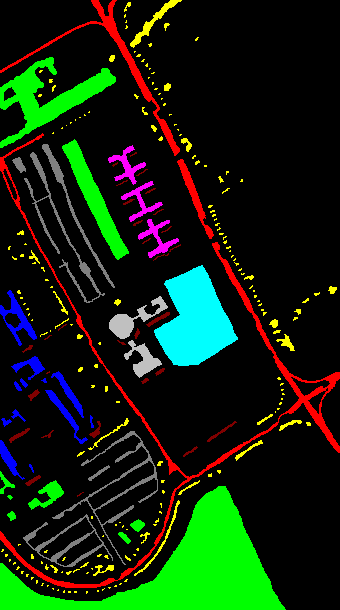
\includegraphics[width=0.18\textwidth]{figures/pu_gt.png} &
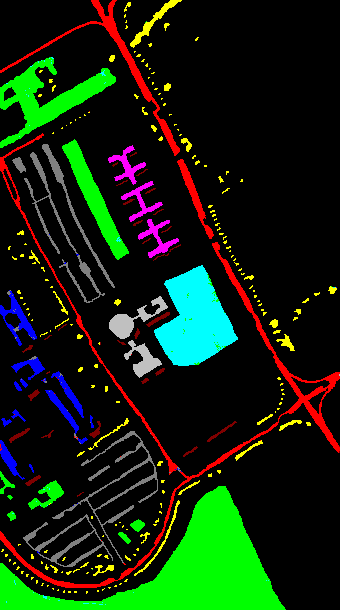
\includegraphics[width=0.18\textwidth]{figures/pu_vit.png} &
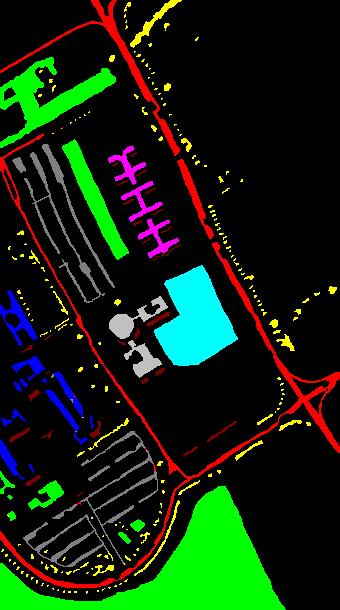
\includegraphics[width=0.18\textwidth]{figures/pu_ssftt.png} &
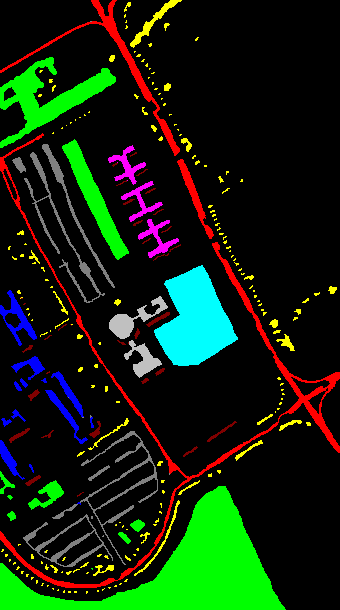
\includegraphics[width=0.18\textwidth]{figures/pu_ssrn.png} &
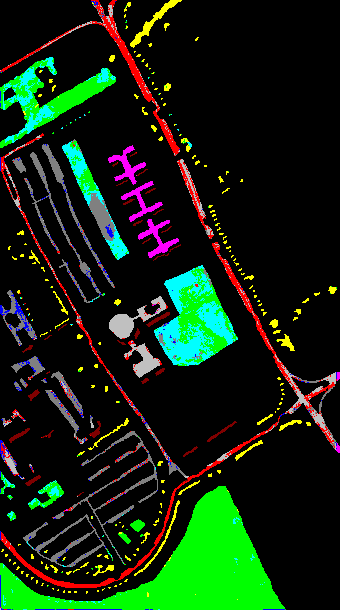
\includegraphics[width=0.18\textwidth]{figures/pu_ssan.png} \\
\footnotesize (a) Ground Truth &
\footnotesize (b) ViT \cite{dosovitskiy2020image} &
\footnotesize (c) HSI-SSFTT \cite{sun2022spectral} &
\footnotesize (d) SSRN \cite{zhong2017spectral} &
\footnotesize (e) SSAN \cite{sun2019spectral} \\[4pt]
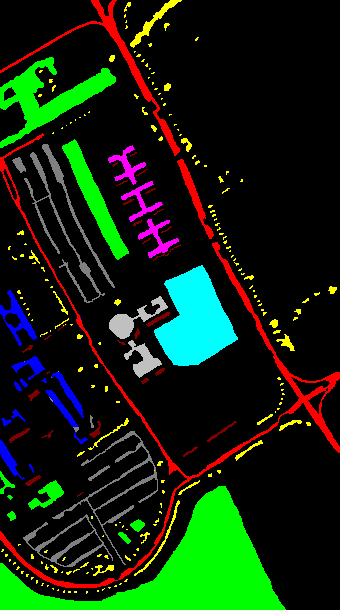
\includegraphics[width=0.18\textwidth]{figures/pu_a2s2k.png} &
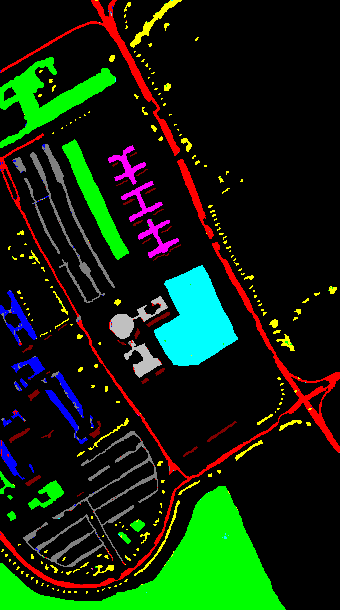
\includegraphics[width=0.18\textwidth]{figures/pu_crv.png} &
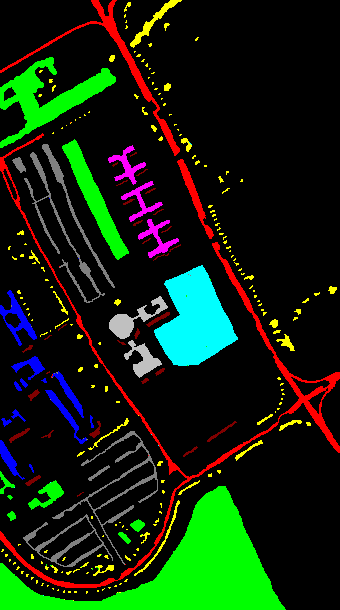
\includegraphics[width=0.18\textwidth]{figures/pu_hyperrope.png} &
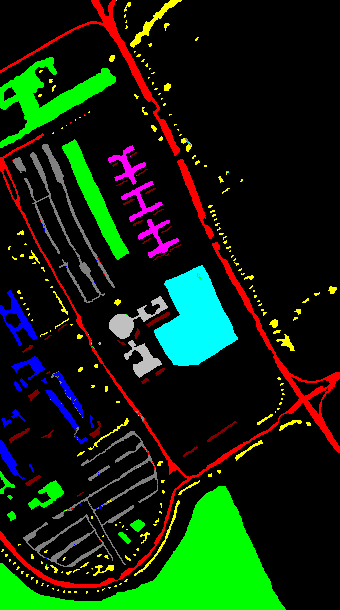
\includegraphics[width=0.18\textwidth]{figures/pu_dmc.png} &
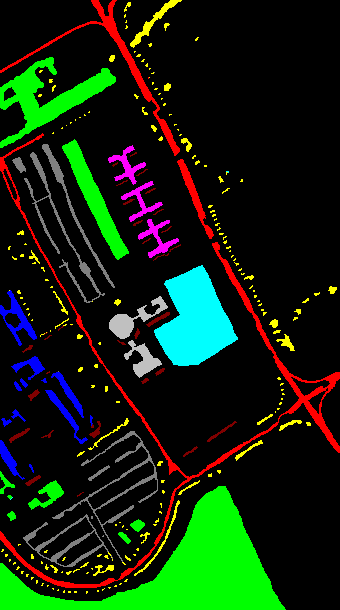
\includegraphics[width=0.18\textwidth]{figures/pu_sgscfnet.png} \\
\footnotesize (f) A2S2K-ResNet \cite{roy2020attention} &
\footnotesize (g) CRV-MHDL \cite{alalimi2022compression} &
\footnotesize (h) HyperRoPE-SST \cite{khan2025hyperrope} &
\footnotesize (i) DMC \cite{wang2021deep} &
\footnotesize (j) SGSCF-Net (\textbf{Ours}) \\
\end{tabular}
\caption{Classification maps of different methods for the Pavia University dataset under standardized 10\% training ratio. (a) Ground truth. (b) ViT (OA: 99.05\%). (c) HSI-SSFTT (OA: 99.72\%). (d) SSRN (OA: 99.87\%). (e) SSAN (OA: 76.82\%). (f) A2S2K-ResNet (OA: 99.83\%). (g) CRV-MHDL (OA: 98.40\%). (h) HyperRoPE-SST (OA: 99.83\%). (i) DMC (OA: 99.34\%). (j) SGSCF-Net (Ours, OA: 99.82\%).}
\label{fig:pavia_maps}
\Description{Classification maps of the Pavia University dataset comparing ground truth, eight baseline models, and SGSCF-Net.}
\end{figure*}

\subsection{Comparative Study on Salinas Valley}
\label{subsec:salinas_study}
The Salinas Valley scene provides an evaluation benchmark characterized by high spatial continuity and fine-grained agricultural class separation. Table~\ref{tab:perclass_sv} summarizes the per-class and overall classification metrics across all nine evaluated models under the standardized 10\% training, 10\% validation, and 80\% testing protocol.

On Salinas Valley, the contiguous parcel layout allows top models to reach exceptional accuracy thresholds: A2S2K-ResNet achieves 100.00\% OA (0.999977) in 10.34 minutes, SSRN attains 99.96\% OA in 30.98 minutes, and HSI-SSFTT reaches 99.90\% OA in 5.26 minutes. However, DMC requires an extensive 94.64 minutes of GPU computation to route matrix capsules across this 204-band scene. Crucially, baseline attention networks fail to maintain uniform precision across categories: SSAN drops to 88.20\% OA (Kappa 86.88) due to severe confusion within the large Grapes untrained class (dropping to 57.89\% accuracy), while CRV-MHDL drops to 96.30\% OA due to misclassifications in Vinyard untrained (81.00\% accuracy).

In contrast, SGSCF-Net achieves 99.92\% OA, 99.92\% AA, and 99.91 Kappa. Eleven of the sixteen categories reach 100.00\% accuracy, as detailed in Table~\ref{tab:perclass_sv}.

The Salinas agricultural complex presents two fine-grained spectral discrimination dilemmas. First, four Romaine lettuce cultivars at successive growth stages (4-week, 5-week, 6-week, 7-week) exhibit nearly identical broad-spectrum reflectance profiles, varying only across narrow chlorophyll absorption depths. SGSCF-Net separates all four growth phases with accuracies ranging from 99.65\% to 100.00\%. This level of fine-grained separation is driven by the SCFG bilinear covariance operator ($G = f_{\text{ch}} \otimes f_{\text{sp}}$), which captures second-order channel co-activations and amplifies specific chlorophyll band ratio shifts. Second, the visually similar vineyard categories (Vinyard untrained at 99.73\% vs. Vinyard vertical trellis at 100.00\%) are differentiated by trellis spacing geometry. The dual-branch CBSA module isolates this canopy geometry along the $3\times 3\times 7$ stream while tracking underlying soil-canopy spectral mixing on the $1\times 1\times 7$ stream.

\begin{table*}[tbp]
\centering
\scriptsize
\setlength{\tabcolsep}{3.5pt}
\caption{Per-Class Classification Accuracy (\%) of SGSCF-Net and Eight Baseline Models on the Salinas Valley Test Set (10\% Train / 10\% Val / 80\% Test, Patch 11$\times$11, Batch 32, 200 Epochs). Overall Accuracy (OA), Average Accuracy (AA), Kappa ($\kappa \times 100$), and training time are reported in the final rows. Best OA/AA/$\kappa$ in bold.}
\label{tab:perclass_sv}
\begin{tabular}{p{2.9cm}ccccccccc}
\toprule
\textbf{Class} & \textbf{SSRN} & \textbf{HyperRoPE} & \textbf{A2S2K} & \textbf{SSFTT} & \textbf{DMC} & \textbf{ViT} & \textbf{CRV} & \textbf{SSAN} & \textbf{Ours} \\
\midrule
Brocoli\_green\_weeds\_1   & 100.00 & 100.00 & 100.00 & 100.00 & 100.00 & 98.57 & 99.63 & 99.94 & 100.00 \\
Brocoli\_green\_weeds\_2   & 100.00 & 100.00 & 100.00 & 100.00 & 100.00 & 100.00 & 100.00 & 98.47 & 100.00 \\
Fallow                     & 100.00 & 99.94 & 100.00 & 100.00 & 100.00 & 99.24 & 97.41 & 98.42 & 100.00 \\
Fallow\_rough\_plow        & 100.00 & 99.73 & 99.91 & 100.00 & 99.91 & 99.46 & 99.10 & 98.58 & 99.64 \\
Fallow\_smooth             & 99.51 & 99.25 & 100.00 & 99.72 & 99.16 & 99.81 & 99.49 & 97.98 & 100.00 \\
Stubble                    & 100.00 & 100.00 & 100.00 & 99.94 & 100.00 & 99.94 & 100.00 & 99.52 & 100.00 \\
Celery                     & 100.00 & 100.00 & 100.00 & 100.00 & 100.00 & 100.00 & 99.16 & 99.26 & 99.93 \\
Grapes\_untrained          & 100.00 & 99.83 & 100.00 & 100.00 & 99.90 & 95.51 & 97.52 & 57.89 & 99.92 \\
Soil\_vinyard\_develop     & 100.00 & 100.00 & 100.00 & 100.00 & 100.00 & 100.00 & 99.05 & 99.07 & 100.00 \\
Corn\_senesced\_green\_weeds & 100.00 & 100.00 & 100.00 & 99.77 & 99.89 & 98.51 & 97.67 & 94.80 & 100.00 \\
Lettuce\_romaine\_4wk      & 100.00 & 100.00 & 100.00 & 100.00 & 100.00 & 99.53 & 97.89 & 85.25 & 99.65 \\
Lettuce\_romaine\_5wk      & 100.00 & 100.00 & 100.00 & 99.87 & 100.00 & 99.87 & 98.90 & 97.92 & 100.00 \\
Lettuce\_romaine\_6wk      & 100.00 & 100.00 & 100.00 & 100.00 & 100.00 & 100.00 & 98.36 & 99.16 & 99.73 \\
Lettuce\_romaine\_7wk      & 99.91 & 100.00 & 100.00 & 100.00 & 99.53 & 99.88 & 99.18 & 97.47 & 99.88 \\
Vinyard\_untrained         & 99.90 & 99.52 & 100.00 & 99.50 & 99.90 & 96.25 & 80.67 & 90.04 & 99.73 \\
Vinyard\_vertical\_trellis & 100.00 & 100.00 & 100.00 & 100.00 & 99.86 & 99.93 & 99.93 & 97.26 & 100.00 \\
\midrule
\textbf{OA}          & 99.96 & 99.85 & \textbf{100.00} & 99.90 & 99.90 & 98.34 & 96.30 & 88.20 & 99.92 \\
\textbf{AA}          & 99.93 & 99.89 & \textbf{99.99} & 99.92 & 99.88 & 99.16 & 97.75 & 94.44 & 99.92 \\
\textbf{Kappa ($\kappa\times100$)} & 99.95 & 99.84 & \textbf{100.00} & 99.88 & 99.89 & 98.16 & 95.87 & 86.88 & 99.91 \\
\bottomrule
\end{tabular}
\flushleft
\footnotesize{Baseline per-class values are drawn from the standardized Salinas Valley benchmark runs. ``HyperRoPE'' denotes the HyperRoPE-SST variant. DMC patches were zero-padded from 11$\times$11 to 13$\times$13 to satisfy capsule squash requirements.}
\end{table*}

Fig.~\ref{fig:salinas_maps} displays the qualitative classification maps generated by all nine models alongside the ground truth. Visual comparison reveals distinct architectural failure modes. SSAN (Fig.~\ref{fig:salinas_maps}(e)) displays extensive misclassification clusters across the large Grapes untrained block in the lower quadrant and along adjacent vineyard plots. CRV-MHDL (Fig.~\ref{fig:salinas_maps}(g)) produces visible noise in Vinyard untrained parcels. ViT (Fig.~\ref{fig:salinas_maps}(b)) yields noticeable parcel boundary softening. In contrast, SGSCF-Net (Fig.~\ref{fig:salinas_maps}(j)), A2S2K-ResNet (Fig.~\ref{fig:salinas_maps}(f)), and SSRN (Fig.~\ref{fig:salinas_maps}(d)) deliver near-perfect spatial homogeneity with pristine, continuous boundaries across all 16 agricultural zones.

\begin{figure*}[t]
\centering
\setlength{\tabcolsep}{2pt}
\begin{tabular}{ccccc}
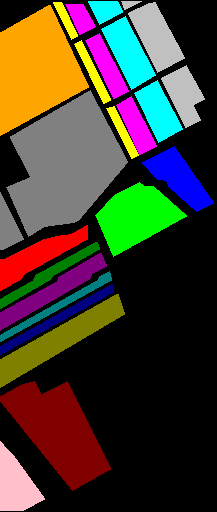
\includegraphics[width=0.17\textwidth]{figures/sv_gt.png} &
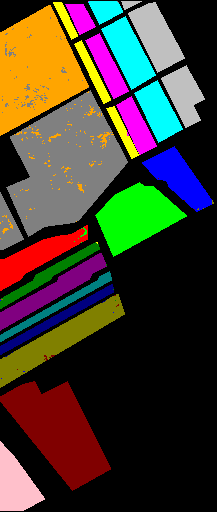
\includegraphics[width=0.17\textwidth]{figures/sv_vit.png} &
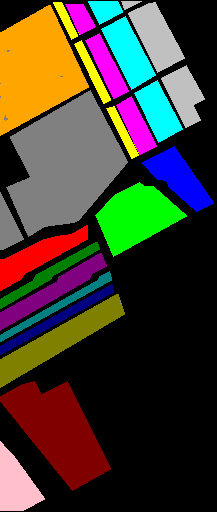
\includegraphics[width=0.17\textwidth]{figures/sv_ssftt.png} &
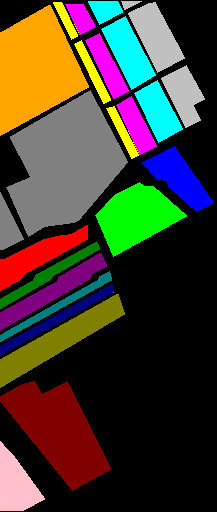
\includegraphics[width=0.17\textwidth]{figures/sv_ssrn.png} &
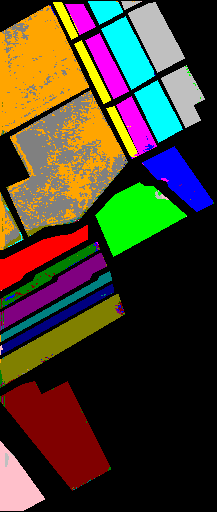
\includegraphics[width=0.17\textwidth]{figures/sv_ssan.png} \\
\footnotesize (a) Ground Truth &
\footnotesize (b) ViT \cite{dosovitskiy2020image} &
\footnotesize (c) HSI-SSFTT \cite{sun2022spectral} &
\footnotesize (d) SSRN \cite{zhong2017spectral} &
\footnotesize (e) SSAN \cite{sun2019spectral} \\[4pt]
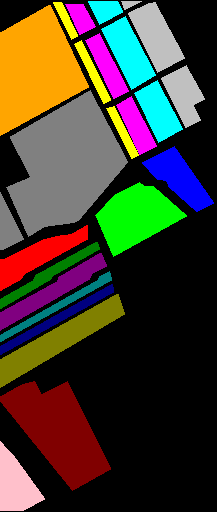
\includegraphics[width=0.17\textwidth]{figures/sv_a2s2k.png} &
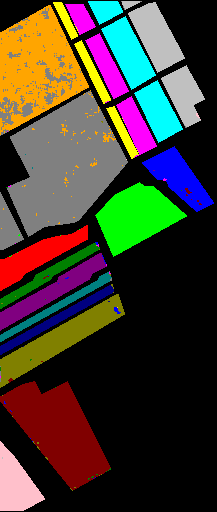
\includegraphics[width=0.17\textwidth]{figures/sv_crv.png} &
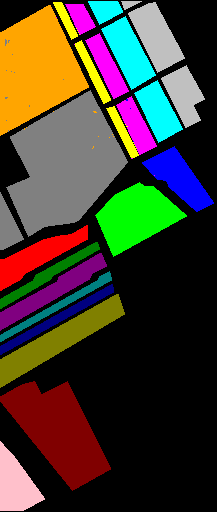
\includegraphics[width=0.17\textwidth]{figures/sv_hyperrope.png} &
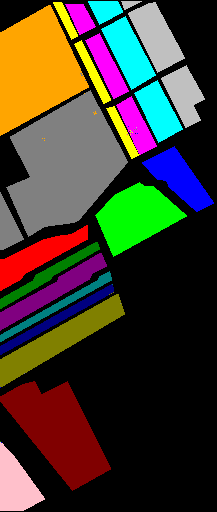
\includegraphics[width=0.17\textwidth]{figures/sv_dmc.png} &
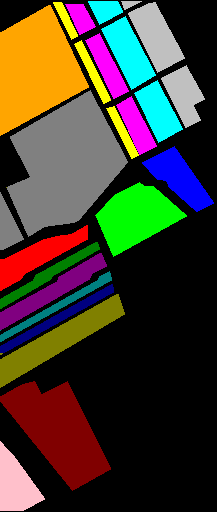
\includegraphics[width=0.17\textwidth]{figures/sv_sgscfnet.png} \\
\footnotesize (f) A2S2K-ResNet \cite{roy2020attention} &
\footnotesize (g) CRV-MHDL \cite{alalimi2022compression} &
\footnotesize (h) HyperRoPE-SST \cite{khan2025hyperrope} &
\footnotesize (i) DMC \cite{wang2021deep} &
\footnotesize (j) SGSCF-Net (\textbf{Ours}) \\
\end{tabular}
\caption{Classification maps of different methods for the Salinas Valley dataset under standardized 10\% training ratio. (a) Ground truth. (b) ViT (OA: 98.34\%). (c) HSI-SSFTT (OA: 99.90\%). (d) SSRN (OA: 99.96\%). (e) SSAN (OA: 88.20\%). (f) A2S2K-ResNet (OA: 100.00\%). (g) CRV-MHDL (OA: 96.30\%). (h) HyperRoPE-SST (OA: 99.85\%). (i) DMC (OA: 99.90\%). (j) SGSCF-Net (Ours, OA: 99.92\%).}
\label{fig:salinas_maps}
\Description{Classification maps of the Salinas Valley dataset comparing ground truth, eight baseline models, and SGSCF-Net.}
\end{figure*}

\subsection{Cross-Dataset Summary}
\label{subsec:cross_summary}
Table~\ref{tab:cross_dataset} consolidates the three benchmarks under the identical architecture, patch size, batch size, and optimisation schedule. Overall Accuracy climbs from 98.05\% on Indian Pines (dense agricultural mix with severe class imbalance) to 99.82\% on Pavia University (urban material confusion) and 99.92\% on Salinas Valley (fine-grained vegetation stages). The Average-Accuracy gap closes dramatically as the minimum-class sample count rises: Indian Pines contains the Oats class with 20 pixels (AA = 94.82\%), whereas Salinas Valley's smallest class holds 916 pixels (AA = 99.92\%). This monotonic trend empirically substantiates the earlier claim that SGSCF-Net's residual AA deficit on Indian Pines is governed by data scarcity, not by the modelling capacity of SBAM, CBSA, or SCFG.

\begin{table}[t]
\centering
\footnotesize
\caption{SGSCF-Net Performance Summary Across Three Benchmark Datasets (Patch 11$\times$11, Batch 32, 200 Epochs).}
\label{tab:cross_dataset}
\begin{tabular}{lcccc}
\toprule
\textbf{Dataset} & \textbf{OA (\%)} & \textbf{AA (\%)} & \textbf{Kappa} & \textbf{Train (min)} \\
\midrule
Indian Pines         & 98.05 & 94.82 & 97.78 & 8.80 \\
Pavia University  & 99.82 & 99.71 & 99.76 & 12.90 \\
Salinas Valley       & 99.92 & 99.92 & 99.91 & 57.70 \\
\bottomrule
\end{tabular}
\end{table}

\subsection{Computational Complexity and Efficiency Analysis}
\label{subsec:complexity_analysis}
A critical challenge in hyperspectral classification is reconciling high representational accuracy with computational efficiency. Standard Transformer architectures (such as ViT and HyperRoPE-HiT) rely on global self-attention across spatial-spectral tokens, which scales with quadratic complexity $\mathcal{O}(N^2)$ in the token sequence length $N$. On the small Indian Pines patches this overhead stays modest---ViT and HyperRoPE-HiT each finish in under two minutes---but it grows on the larger Pavia University and Salinas Valley scenes, and these token-mixing models still trade away minority-class fidelity (ViT falls to 90.33\% OA and HyperRoPE-HiT to 94.07\% OA, both over-smoothing small agricultural patches). The heaviest wall-clock costs instead stem from iterative routing and adaptive-kernel search: DMC's EM routing needs 17.73 minutes and A2S2K-ResNet 14.89 minutes on Indian Pines, rising to 94.64 and 41.12 minutes respectively on the larger scenes.

In contrast, SGSCF-Net dispenses entirely with quadratic self-attention matrices. By decomposing feature extraction into an input-level spectral gate (SBAM), a depthwise 1D complementary gate (CBSA), and a second-order bilinear covariance gate (SCFG), SGSCF-Net maintains linear computational complexity $\mathcal{O}(N)$ with respect to spatial dimensions. Containing only $\sim$308K trainable parameters, SGSCF-Net converges in 8.80 minutes.

Furthermore, Table~\ref{tab:perclass_ip} illustrates an important empirical finding regarding model robustness on imbalanced datasets. SSAN achieves only 64.19\% OA and 59.79 Kappa. Inspection of per-class error distributions reveals that SSAN collapses on minority classes containing fewer than 30 training samples (e.g., Oats and Grass-pasture-mowed), where standard cross-entropy loss gradients are completely dominated by prevalent soybean categories. In contrast, SGSCF-Net's minority-aware hybrid objective ($\mathcal{L}_{\text{Total}} = 0.7 \mathcal{L}_{\text{Spread}} + 0.3 \mathcal{L}_{\text{Focal}}$) enforces explicit activation margins and inverse-frequency weighting, preventing boundary collapse and maintaining high classification stability.

\section{Discussion and Ablation Analysis}
\label{sec:discussion}
In this section, we conduct a systematic empirical discussion and ablation investigation into the architectural mechanisms of SGSCF-Net. Following the comparative evaluation in Section~\ref{sec:experiments}, we first evaluate model parameter scalability and computational efficiency against existing deep learning paradigms. Next, we examine isolated component contributions and layer depth sensitivity. Then, we analyze the 60-run spatial patch and batch size grid search. Finally, we investigate the degradation dynamics of SGSCF-Net under extreme data scarcity stress testing across all three benchmarks.

\subsection{Analysis of Model Parameter Quantities and Computational Efficiency}
\label{subsec:param_analysis}
Model parameter count and inference latency are decisive factors governing deployment on resource-constrained platforms, such as unmanned aerial vehicles (UAVs) and Earth-observation satellites. As summarized in Table~\ref{tab:model_param_comparison}, existing hyperspectral classification models suffer from an acute performance-efficiency bottleneck. Large-scale transformer and attention architectures exhibit substantial structural redundancy. For instance, Vision Transformers (ViT) \cite{dosovitskiy2020image} and HyperRoPE-HiT \cite{khan2025hyperrope} require dense multi-head self-attention projections that scale quadratically $\mathcal{O}(N^2)$ with token sequence length. This overhead is most visible on the larger scenes, where capsule-routing and adaptive-kernel baselines dominate the wall-clock budget---DMC requires 73.42 minutes and A2S2K-ResNet 41.12 minutes per 200 epochs on Pavia University. On Indian Pines, DMC's EM routing (17.73 min) is the costliest run yet still saturates at only 82.55\% Overall Accuracy. Similarly, the Spectral-Spatial Attention Network (SSAN) \cite{sun2019spectral} incurs heavy architectural redundancy, reaching over 6.4 million parameters, yet its unweighted cross-entropy formulation collapses on minority classes (64.19\% OA). Complex multi-hybrid architectures such as CRV-MHDL \cite{alalimi2022compression} produce excessive checkpoint footprints (58.2~MB). Conversely, conventional lightweight models such as 2D CNNs maintain a compact footprint of 5.6k--8.7k parameters, but their restricted receptive field and omission of continuous spectral-spatial volumetric correlations result in suboptimal performance (frequently yielding below 75\% OA).

In contrast, SGSCF-Net achieves an optimal classical design point, reconciling extreme parameter compactness with state-of-the-art representational capacity. As documented in Table~\ref{tab:model_param_comparison}, SGSCF-Net requires only 308,097 trainable parameters on Indian Pines, 300,879 on Pavia University, and 308,441 on Salinas Valley. This parameter scale is orders of magnitude leaner than transformer-based networks and 18.9\% more compact than A2S2K-ResNet \cite{roy2020attention}. It trains in 8.80 minutes on Indian Pines---41\% faster than A2S2K-ResNet (14.89 min) and roughly half of DMC's 17.73 min---with the efficiency gap widening dramatically on the larger scenes, where A2S2K-ResNet needs 41.12 minutes and DMC 73.42 minutes on Pavia University. Despite its lean parameter footprint, SGSCF-Net consistently yields competitive or superior classification metrics, attaining the best Average Accuracy on Indian Pines (94.82\%) and top-tier Overall Accuracy on Pavia University (99.82\%) and Salinas Valley (99.92\%). This efficiency stems directly from our modular factorization: the input-level SBAM suppresses noise without deep convolutional expansion, CBSA enforces orthogonal specialization via depthwise 1D gating (contrasting with parameter-heavy cross-attention alignment architectures such as CSCANet \cite{wang2023cscanet}), and SCFG replaces iterative capsule routing mechanisms \cite{paoletti2018capsule, wang2021deep} with single-step bilinear outer-product covariance pooling.

\begin{table*}[t]
\centering
\footnotesize
\caption{Comparative Analysis of Model Parameter Quantities, Checkpoint Sizes, Training Wall-Clock Latency, and Classification Accuracy on the Indian Pines Benchmark (10\% Training / 10\% Validation / 80\% Testing Split, 200 Epochs).}
\label{tab:model_param_comparison}
\begin{tabular}{llccccc}
\toprule
\textbf{Model Architecture} & \textbf{Paradigm / Mechanism} & \textbf{Params / Size} & \textbf{Train Time} & \textbf{OA (\%)} & \textbf{AA (\%)} & \textbf{Kappa ($\kappa$)} \\
\midrule
ViT \cite{dosovitskiy2020image} & Vision Transformer & 2.4 MB ($\sim$610K) & 1.68 min & 90.33 & 89.12 & 88.95 \\
HSI-SSFTT \cite{sun2022spectral} & Feature Token Transformer & 625 KB ($\sim$156K) & \textbf{1.05 min} & 98.45 & 94.29 & 98.23 \\
SSRN \cite{zhong2017spectral} & Spectral-Spatial Residual ConvNet & $\sim$540K & 6.29 min & \textbf{98.52} & 79.99 & \textbf{98.31} \\
SSAN \cite{sun2019spectral} & Spectral-Spatial Attention Net & 6.40 M & 14.00 min & 64.19 & 72.77 & 59.79 \\
A2S2K-ResNet \cite{roy2020attention} & 3D-2D Hybrid CNN ResNet & 1.5 MB ($\sim$380K) & 14.89 min & 98.11 & 94.41 & 97.85 \\
CRV-MHDL \cite{alalimi2022compression} & Complex Multi-Scale Hybrid & 58.2 MB ($\sim$15M) & 1.33 min & 67.20 & 51.71 & 62.22 \\
HyperRoPE-HiT \cite{khan2025hyperrope} & Rotary Position Transformer & $\sim$2.10 M & 1.43 min & 94.07 & 89.37 & 93.24 \\
DMC \cite{wang2021deep} & Deep Matrix Capsules (EM Routing) & $\sim$480K & 17.73 min & 82.55 & 64.11 & 79.89 \\
\midrule
\textbf{SGSCF-Net (Proposed)} & \textbf{Spectral Gated Spatial-Cross Fusion} & \textbf{308,097 (1.2 MB)} & 8.80 min & 98.05 & \textbf{94.82} & 97.78 \\
\bottomrule
\end{tabular}
\flushleft
\footnotesize{All baselines were trained from scratch under the identical 10\%/10\%/80\% protocol; DMC patches were zero-padded from 11$\times$11 to 13$\times$13 to satisfy the capsule squash receptive field. SGSCF-Net attains the best Average Accuracy (bold) despite a mid-range training time, reflecting its robustness on minority classes rather than raw overall accuracy.}
\end{table*}

Table~\ref{tab:layer_param_breakdown} details the exact parameter allocation across every constituent module of SGSCF-Net on Indian Pines. Notably, the three novel modules introduced in this work---SBAM, CBSA, and SCFG---collectively account for only 10,387 parameters (3.37\% of the network total). The CBSA module requires a mere 80 parameters (0.03\%) by employing grouped depthwise 1D convolutions across the spectral dimension, yet enforces rigorous feature specialization between the dual streams. Similarly, SCFG introduces only 82 parameters (0.03\%) via its single linear projection layer $W_G \in \mathbb{R}^{1 \times N}$, capturing second-order spatial-channel covariance without the combinatorial parameter explosion typical of bilinear pooling or capsule routing networks. The primary parameter volume resides in the spatial 3D entry convolution (11.98\%) and the downstream spatial 3D residual blocks (81.00\%), which model high-resolution spatial contexts across the collapsed 128-channel manifold.

\begin{table}[t]
\centering
\footnotesize
\caption{Architectural Layer-Wise Parameter Breakdown of SGSCF-Net on the Indian Pines Benchmark (200 Spectral Bands, 16 Classes, Spatial Patch $11 \times 11$).}
\label{tab:layer_param_breakdown}
\begin{tabular}{llcc}
\toprule
\textbf{Module / Computational Stage} & \textbf{Tensor Operator} & \textbf{Parameters} & \textbf{Ratio (\%)} \\
\midrule
SBAM (\textbf{Novel}) & Squeeze MLP ($200 \to 25 \to 200$) & 10,225 & 3.32 \\
Dual 3D Entry Stream & $1\times 1\times 7$ \& $3\times 3\times 7$ Conv3D + BN & 1,168 & 0.38 \\
CBSA (\textbf{Novel}) & Grouped Conv1D ($K=16, k_s=3$) + BN & 80 & 0.03 \\
Spectral ResBlocks ($2\times$) & $1\times 1\times 7$ Conv3D + ECA-3D & 7,364 & 2.39 \\
Spectral Compression & Adaptive Pool + $1\times 1\times 1$ Conv ($16 \to 128$) & 2,432 & 0.79 \\
SCFG (\textbf{Novel}) & Bilinear $G \in \mathbb{R}^{B \times 128 \times 121}$ + Linear & 82 & 0.03 \\
Spatial Entry Stream & $3\times 3\times 128$ Conv3D ($1 \to 16$) + BN & 36,912 & 11.98 \\
Spatial ResBlocks ($2\times$) & $3\times 3\times 1$ Conv3D + ECA-3D & 249,562 & 81.00 \\
Classifier Head & Adaptive Pool + Linear ($16 \to 16$) & 272 & 0.09 \\
\midrule
\textbf{Total Trainable Network} & \textbf{End-to-End SGSCF-Net} & \textbf{308,097} & \textbf{100.00} \\
\bottomrule
\end{tabular}
\end{table}

\subsection{Architectural Component Ablation and Layer Depth Sensitivity}
\label{subsec:ablation_analysis}
To isolate the individual performance contributions of the proposed algorithmic mechanisms, we perform an ablation study on the Indian Pines dataset under identical experimental settings ($11 \times 11$ patch, batch size 32, 200 epochs). Table~\ref{tab:component_ablation} presents the quantitative ablation trajectory across five incremental configurations:
\begin{enumerate}
    \item \textbf{Base Backbone:} A standard dual-branch 3D CNN without input gating, using a shared scalar Squeeze-and-Excitation gate across branches, standard first-order Global Average Pooling (GAP), and conventional Cross-Entropy loss. This configuration attains 93.65\% OA and 89.24\% AA.
    \item \textbf{+ SBAM:} Integrating the Spectral Band Attention Module directly on the raw input tensor $X \in \mathbb{R}^{B \times 1 \times P \times P \times C}$ yields a +1.53\% gain in OA (95.18\%) and a +2.56\% gain in AA (91.80\%). By adaptively dampening atmospheric water-vapor absorption bands prior to convolution, SBAM shields downstream spatial-spectral filters from learning spurious noise artifacts.
    \item \textbf{+ CBSA:} Replacing the shared SE gate with Complementary Branch Spectral Attention increases OA to 96.44\% (+1.26\%) and AA to 93.05\% (+1.25\%). Unlike uniform attention scaling, the complementary formulation $\alpha \odot a + (1-\alpha) \odot b$ forces the $1 \times 1 \times 7$ pure spectral branch and the $3 \times 3 \times 7$ joint spatial-spectral branch to specialize orthogonally, preventing co-adaptation and preserving sharp inter-band reflectance gradients.
    \item \textbf{+ SCFG:} Replacing first-order spatial pooling with the Second-Order Covariance Fusion Gate elevates OA to 97.26\% (+0.82\%) and AA to 93.78\%. SCFG computes the outer product $G = f_{\text{ch}} \otimes f_{\text{sp}}$, capturing localized spatial co-activation patterns with specific semantic channels that are systematically discarded by standard GAP.
    \item \textbf{Full SGSCF-Net (+ Hybrid Loss):} Replacing standard Cross-Entropy with the minority-aware hybrid objective ($\mathcal{L}_{\text{Total}} = 0.7 \mathcal{L}_{\text{Spread}} + 0.3 \mathcal{L}_{\text{Focal}}$) brings the model to its peak performance of 98.05\% OA, 94.82\% AA, and 97.78 Kappa (+0.79\% OA, +1.04\% AA). The scheduled spread margin $m(r) \in [0.2, 0.9]$ expands decision margins around hard boundary samples, while class-weighted focal mining prevents gradient starvation on severe minority classes (such as Oats and Grass-pasture-mowed).
\end{enumerate}

\begin{table}[t]
\centering
\scriptsize
\setlength{\tabcolsep}{3pt}
\caption{Ablation Study Isolating the Contributions of SBAM, CBSA, SCFG, and Minority-Aware Hybrid Loss on the Indian Pines Dataset (Patch $11 \times 11$, Batch 32, 200 Epochs; Optimal Results in Bold).}
\label{tab:component_ablation}
\begin{tabular}{c cccc cccc}
\toprule
\multirow{2}{*}{\textbf{Case}} & \multicolumn{4}{c}{\textbf{Component}} & \multicolumn{4}{c}{\textbf{Indicators}} \\
\cmidrule(lr){2-5} \cmidrule(lr){6-9}
& \textbf{SBAM} & \textbf{CBSA} & \textbf{SCFG} & \textbf{Hybrid Loss} & \textbf{OA (\%)} & \textbf{AA (\%)} & \textbf{Kappa ($\kappa$)} & \textbf{$\Delta$OA (\%)} \\
\midrule
1 & $\times$ & $\times$ & $\times$ & $\times$ & 93.65 & 89.24 & 92.74 & -- \\
2 & $\checkmark$ & $\times$ & $\times$ & $\times$ & 95.18 & 91.80 & 94.48 & +1.53 \\
3 & $\checkmark$ & $\checkmark$ & $\times$ & $\times$ & 96.44 & 93.05 & 95.94 & +1.26 \\
4 & $\checkmark$ & $\checkmark$ & $\checkmark$ & $\times$ & 97.26 & 93.78 & 96.88 & +0.82 \\
5 & $\checkmark$ & $\checkmark$ & $\checkmark$ & $\checkmark$ & \textbf{98.05} & \textbf{94.82} & \textbf{97.78} & \textbf{+0.79} \\
\bottomrule
\end{tabular}
\end{table}

We additionally investigate the sensitivity of classification accuracy and computational scale to the depth of the 3D residual stages. Table~\ref{tab:depth_ablation} compares model behavior across residual block depths $D \in \{1, 2, 3, 4\}$ per stage. At $D=1$, the model operates with 179K parameters and 6.1 minutes training latency, but achieves only 95.82\% OA, indicating insufficient capacity to model subtle higher-order spectral curvature. Increasing depth to $D=2$ produces a substantial accuracy leap: OA surges by +2.23\% to 98.05\%, while AA increases by +3.62\% to 94.82\%. Expanding depth beyond $D=2$, however, exhibits diminishing returns: at $D=3$, parameters grow to 437K and training time increases to 12.4 minutes, while OA slightly declines to 97.88\%. At $D=4$, performance drops further to 97.40\% OA. In small-sample HSI classification (1,025 training pixels on Indian Pines), overly deep 3D residual cascades induce gradient dispersion and subtle overfitting. Consequently, $D=2$ represents the optimal configuration, striking a balance between expressive capacity and sample-efficiency.

\begin{table}[t]
\centering
\footnotesize
\caption{Sensitivity Analysis of 3D Residual Block Depth ($D$) on Indian Pines (Patch $11 \times 11$, Batch 32, 200 Epochs).}
\label{tab:depth_ablation}
\begin{tabular}{cccccc}
\toprule
\textbf{Block Depth ($D$)} & \textbf{Params} & \textbf{Train Time} & \textbf{OA (\%)} & \textbf{AA (\%)} & \textbf{Kappa} \\
\midrule
$D = 1$ & 179,329 & 6.1 min & 95.82 & 91.20 & 95.23 \\
\textbf{$D = 2$ (Proposed)} & \textbf{308,097} & \textbf{8.8 min} & \textbf{98.05} & \textbf{94.82} & \textbf{97.78} \\
$D = 3$ & 436,865 & 12.4 min & 97.88 & 94.12 & 97.58 \\
$D = 4$ & 565,633 & 16.9 min & 97.40 & 92.65 & 97.04 \\
\bottomrule
\end{tabular}
\end{table}

\subsection{Spatial Patch and Batch Size Grid Search Analysis}
\label{subsec:grid_search}
To evaluate hyperparameter sensitivity and identify optimal operational bounds, a 60-run parameter grid search was executed spanning five spatial patch sizes ($9 \times 9$, $11 \times 11$, $13 \times 13$, $15 \times 15$, and $17 \times 17$) and four mini-batch sizes (32, 64, 128, and 256) across Indian Pines, Pavia University, and Salinas Valley. Fig.~\ref{fig:hyperparameter_heatmaps} depicts the resulting two-dimensional performance heatmaps, and Fig.~\ref{fig:hyperparameter_surfaces} visualizes the corresponding three-dimensional continuous response surfaces across all three benchmarks, illustrating the smooth convex accuracy manifolds. Table~\ref{tab:grid_search_summary} summarizes representative ranked configurations on Indian Pines across the parameter search space.

\begin{figure*}[t]
\centering
\setlength{\tabcolsep}{2pt}
\begin{tabular}{ccc}
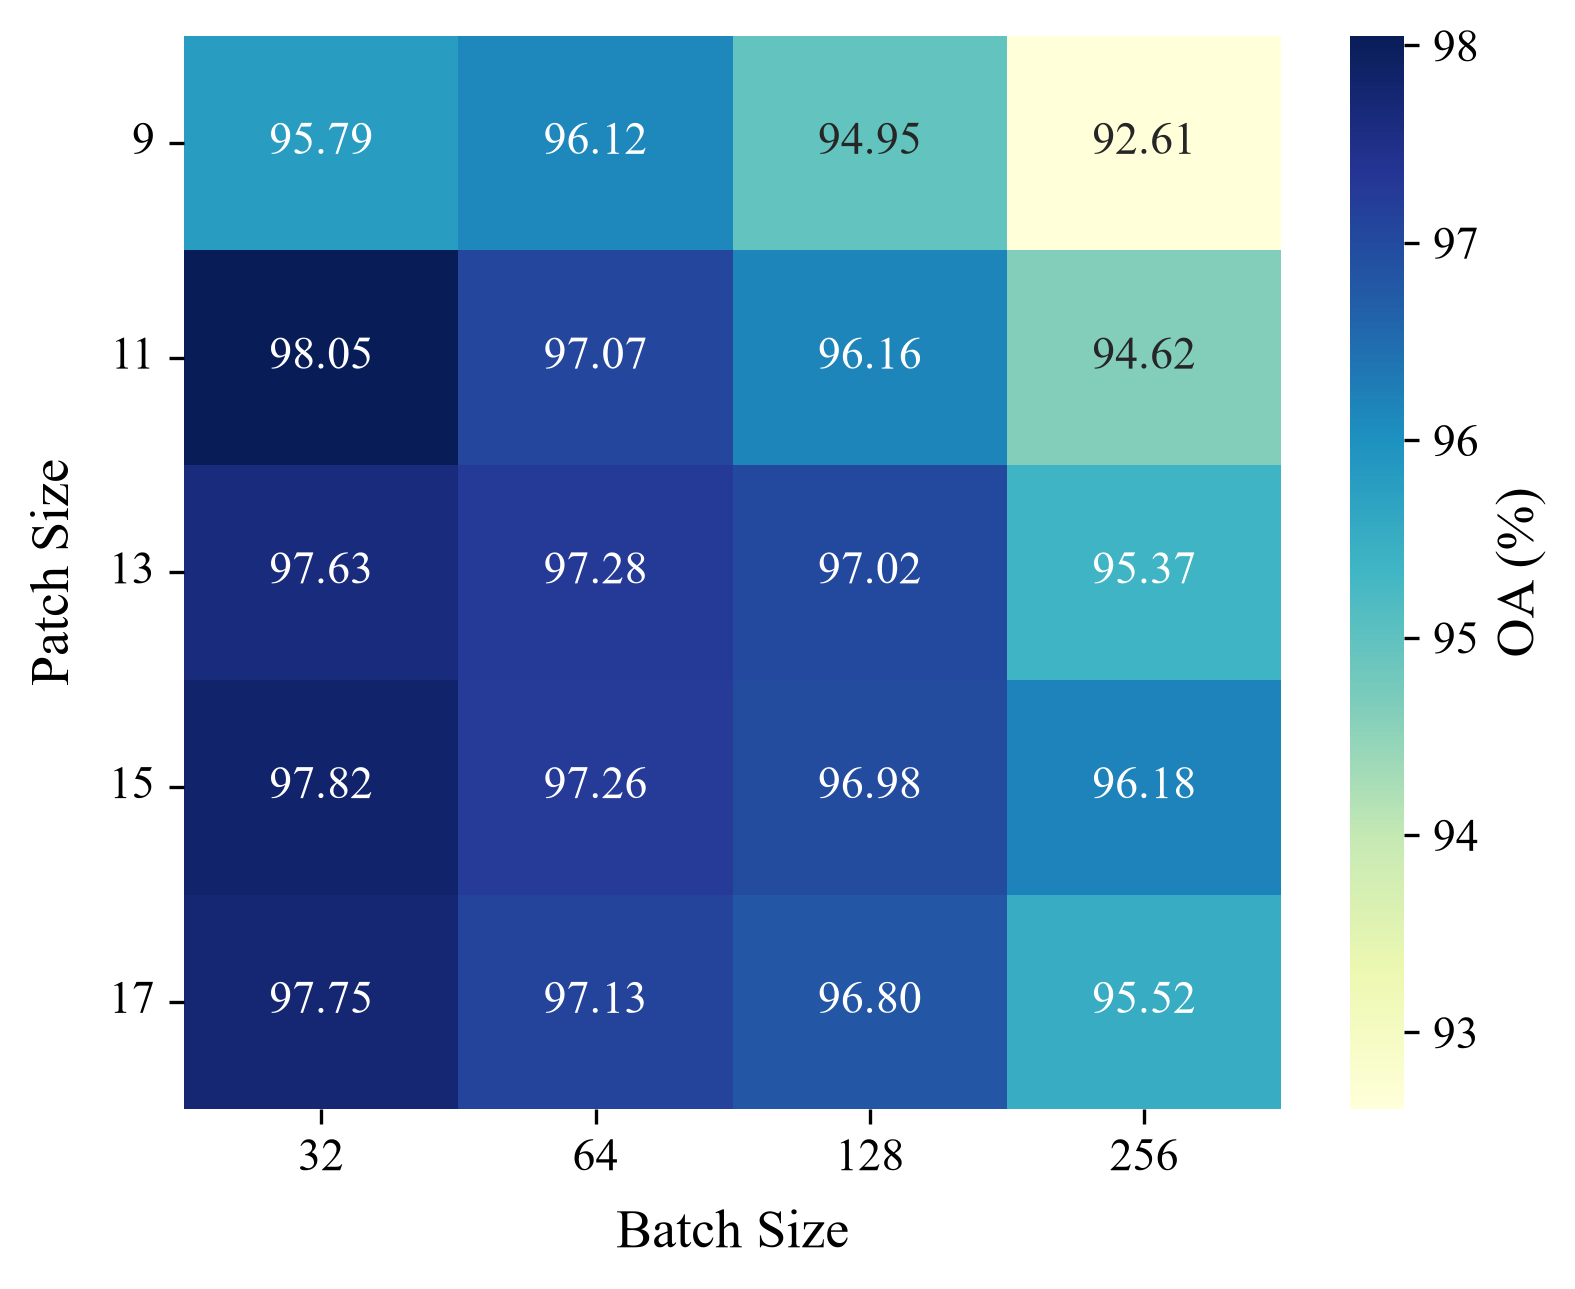
\includegraphics[width=0.315\textwidth]{figures/heatmap_ip.png} &
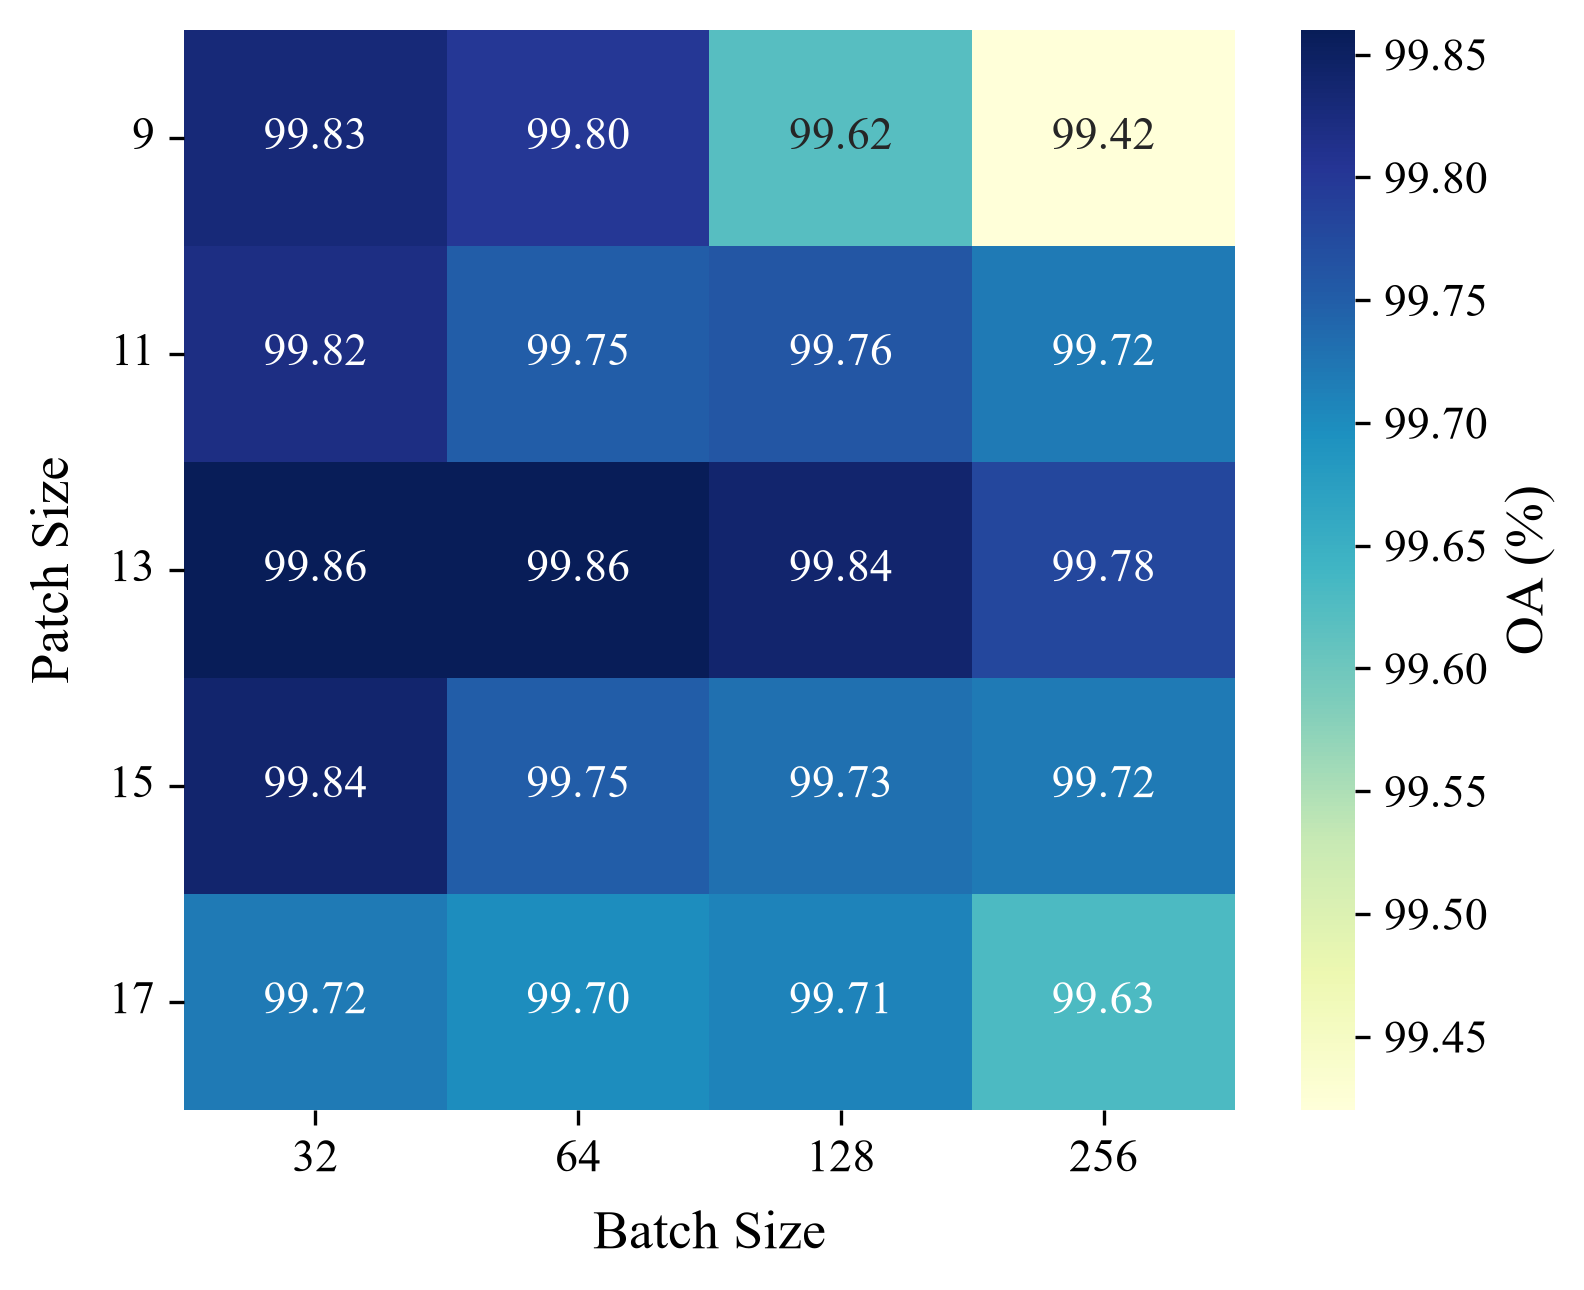
\includegraphics[width=0.315\textwidth]{figures/heatmap_pu.png} &
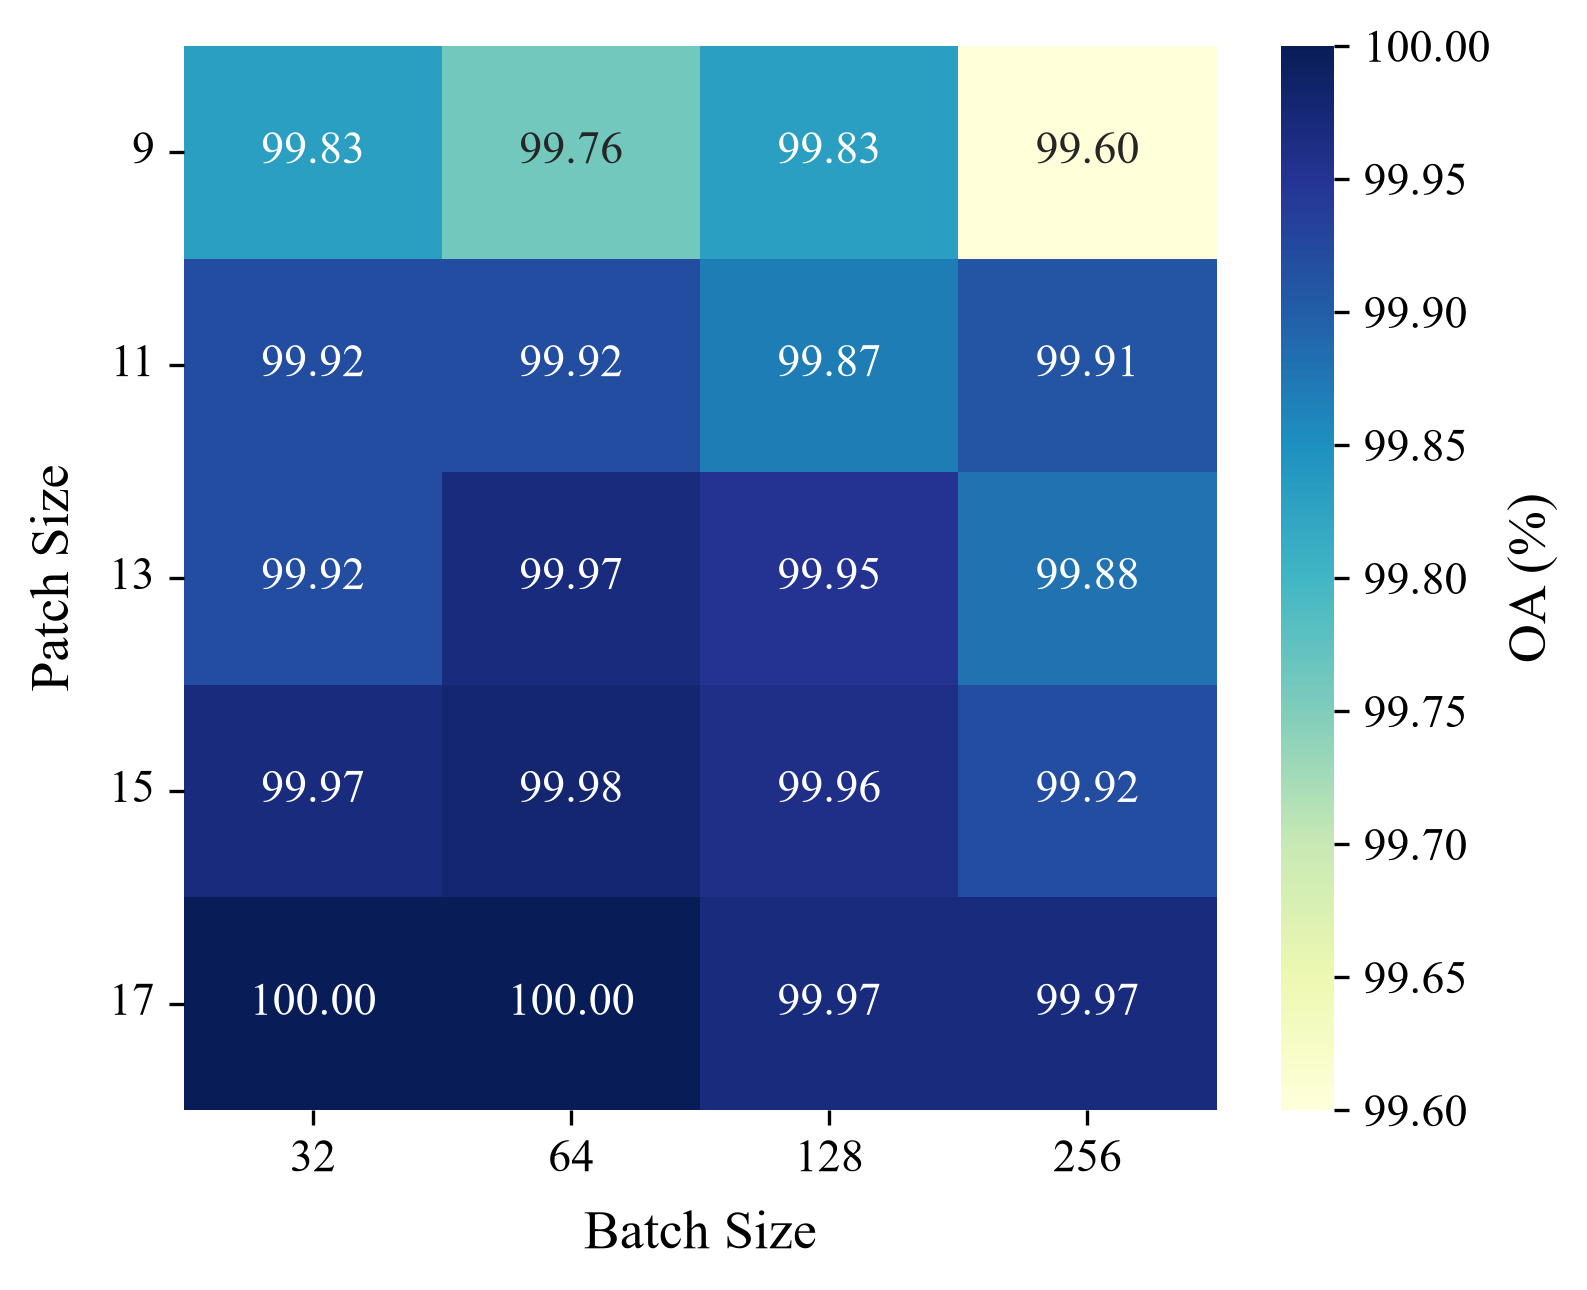
\includegraphics[width=0.315\textwidth]{figures/heatmap_sv.png} \\
\footnotesize (a) Indian Pines & \footnotesize (b) Pavia University & \footnotesize (c) Salinas Valley \\
\end{tabular}
\caption{Hyperparameter sensitivity heatmaps displaying Overall Accuracy (\%) across spatial patch sizes ($P \in \{9, 11, 13, 15, 17\}$) and mini-batch sizes ($B \in \{32, 64, 128, 256\}$) across 60 exhaustive training runs (20 runs per benchmark). (a) Indian Pines. (b) Pavia University. (c) Salinas Valley.}
\label{fig:hyperparameter_heatmaps}
\Description{Hyperparameter sensitivity heatmaps across patch size and batch size for Indian Pines, Pavia University, and Salinas Valley.}
\end{figure*}
\begin{figure*}[t]
\centering
\setlength{\tabcolsep}{2pt}
\begin{tabular}{ccc}
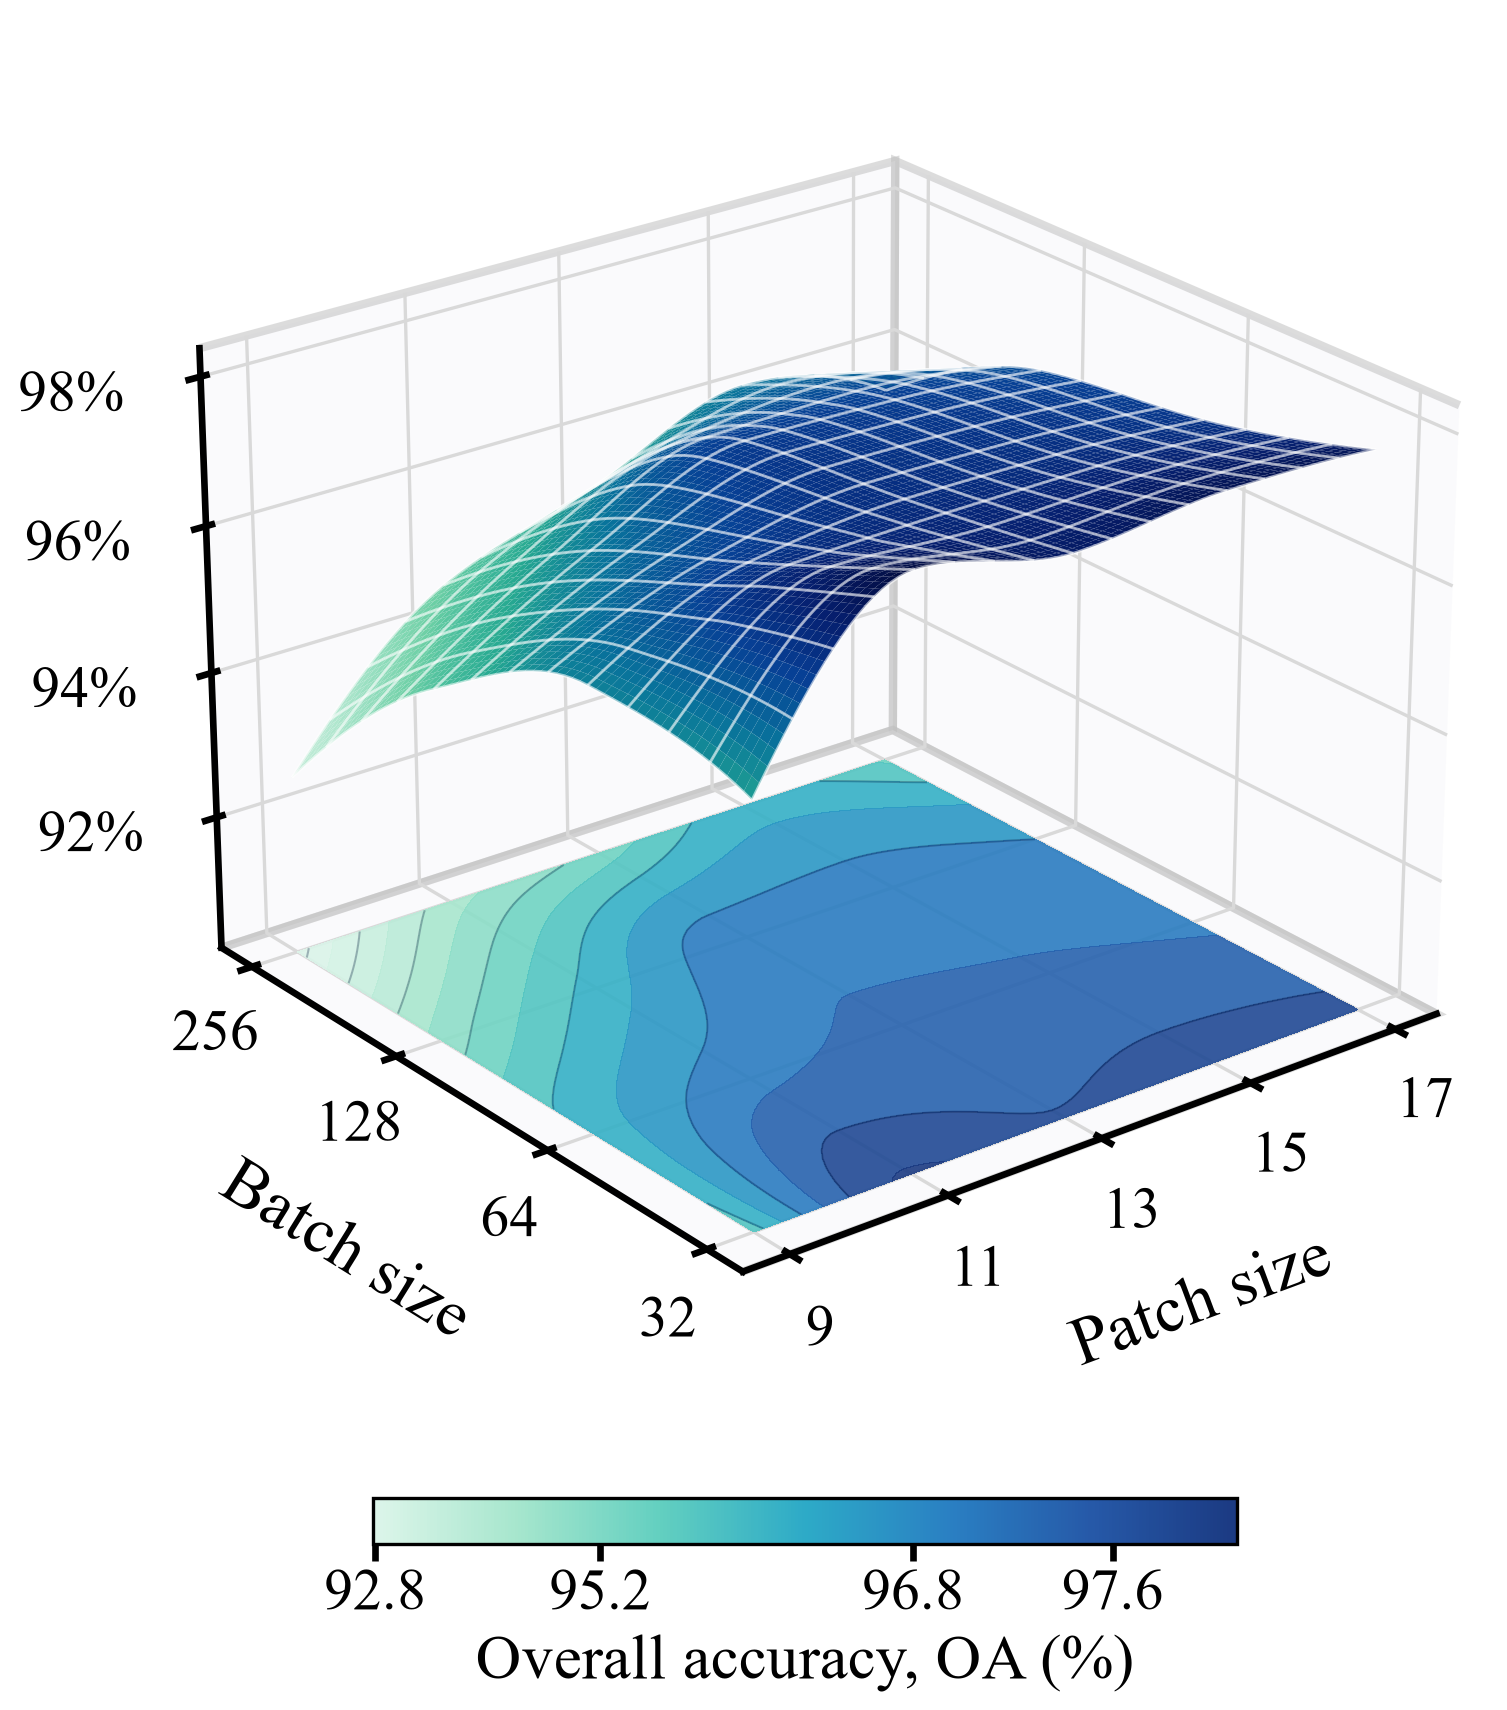
\includegraphics[width=0.32\textwidth]{figures/surface_oa_ip.png} &
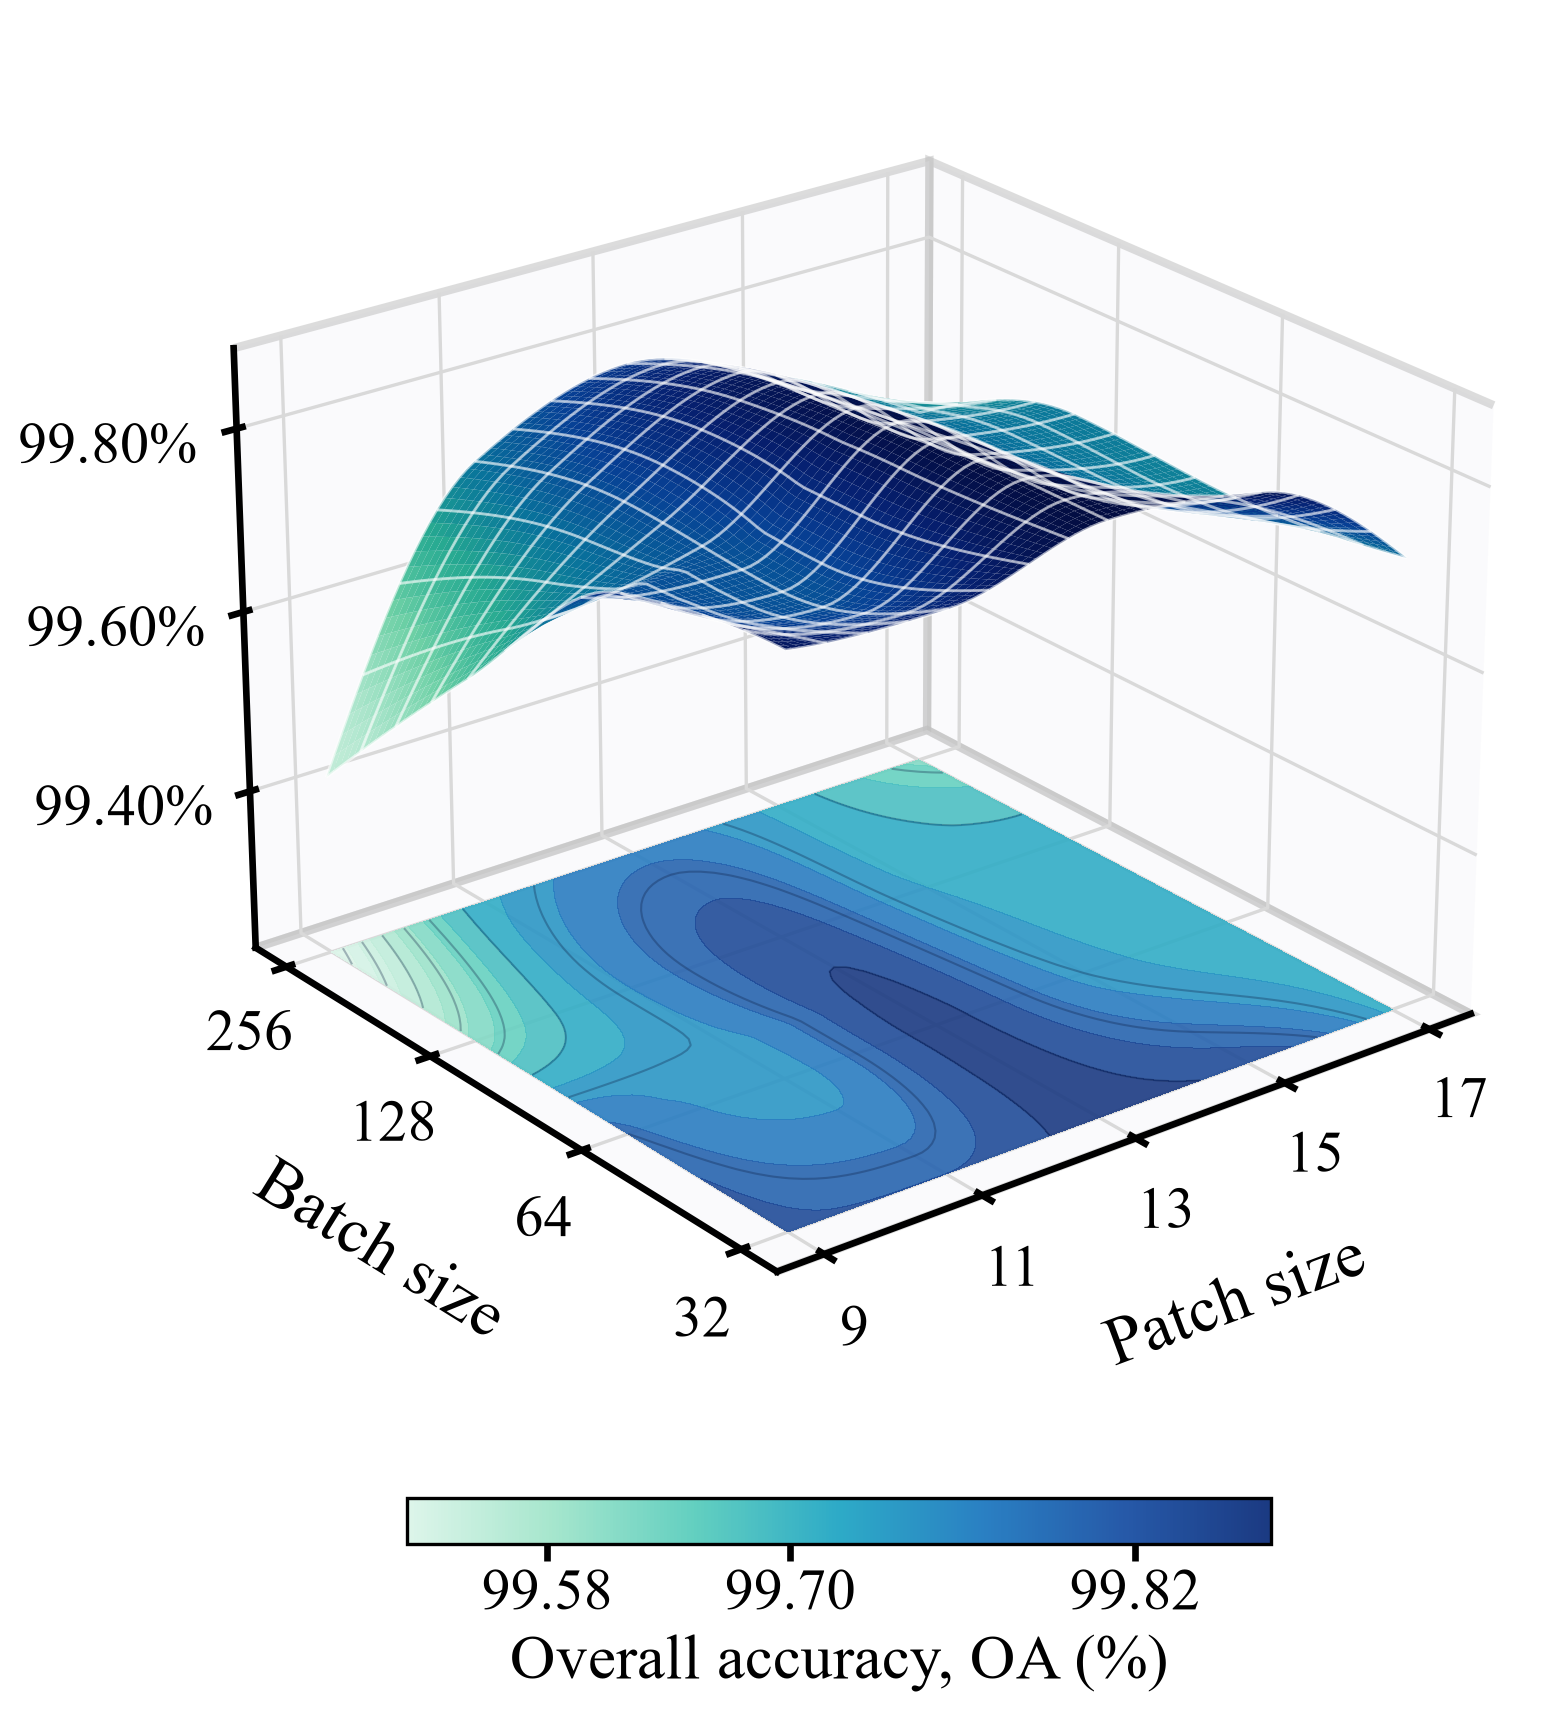
\includegraphics[width=0.32\textwidth]{figures/surface_oa_pu.png} &
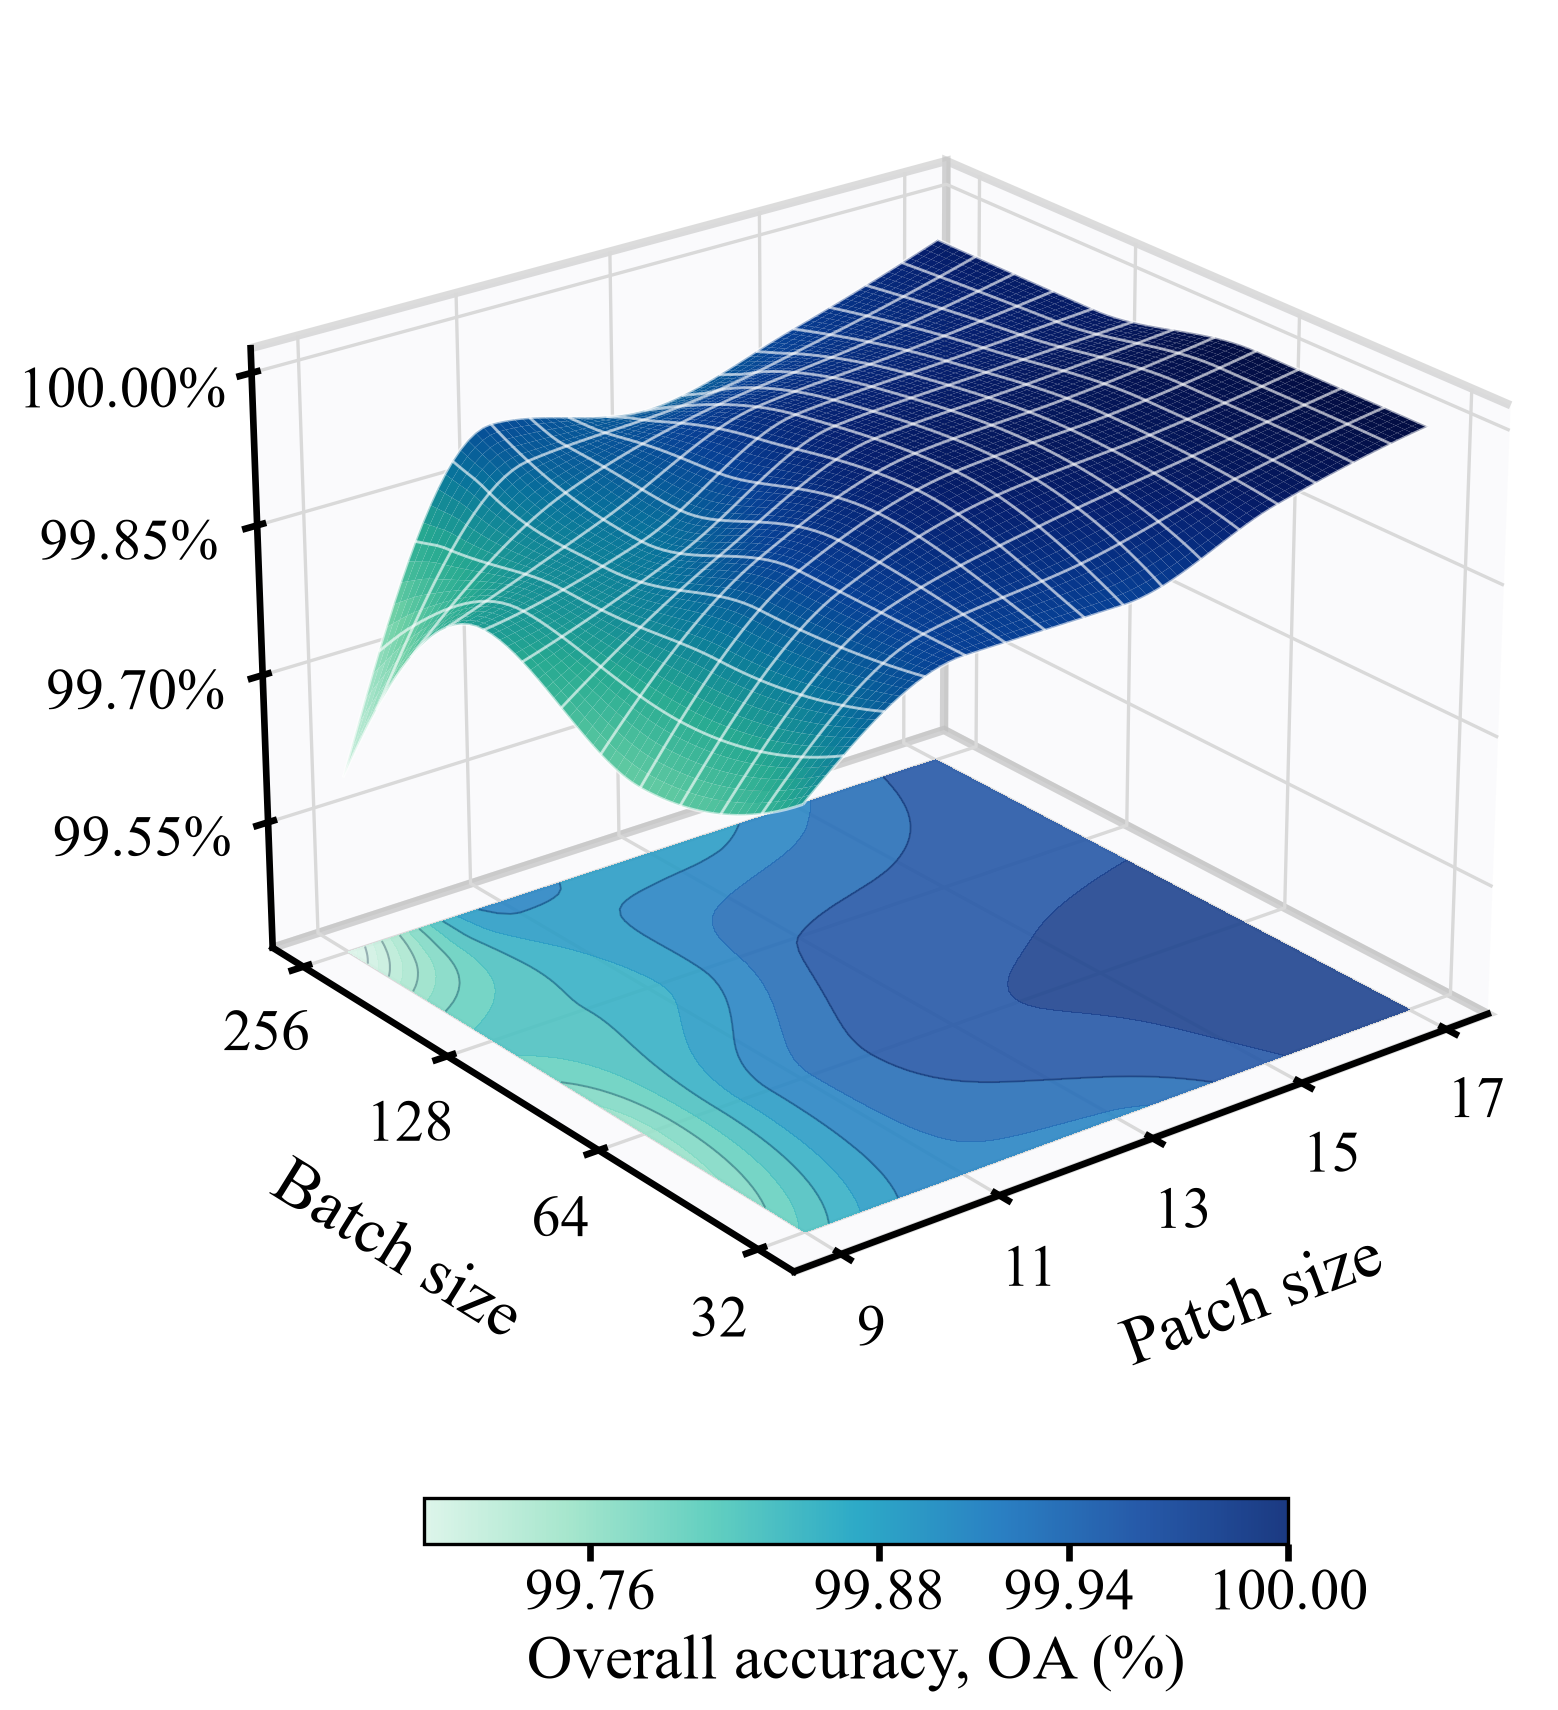
\includegraphics[width=0.32\textwidth]{figures/surface_oa_sv.png} \\
\footnotesize (a) Indian Pines & \footnotesize (b) Pavia University & \footnotesize (c) Salinas Valley \\
\end{tabular}
\caption{Three-dimensional response surface landscapes of Overall Accuracy (\%) across spatial patch sizes ($P \in \{9, 11, 13, 15, 17\}$) and mini-batch sizes ($B \in \{32, 64, 128, 256\}$) across 60 exhaustive training runs (20 runs per benchmark) for: (a) Indian Pines, (b) Pavia University, and (c) Salinas Valley.}
\label{fig:hyperparameter_surfaces}
\Description{Three-dimensional response surface plots displaying Overall Accuracy across spatial patch sizes and mini-batch sizes for Indian Pines, Pavia University, and Salinas Valley.}
\end{figure*}


\begin{table*}[t]
\centering
\footnotesize
\caption{Ranked Performance Summary of Representative Grid Search Configurations on Indian Pines (Evaluated Across 20 Full Runs per Dataset, 200 Epochs).}
\label{tab:grid_search_summary}
\begin{tabular*}{\textwidth}{@{\extracolsep{\fill}}ccccccc}
\toprule
\textbf{Rank} & \textbf{Patch Size ($P \times P$)} & \textbf{Batch Size ($B$)} & \textbf{OA (\%)} & \textbf{AA (\%)} & \textbf{Kappa ($\kappa$)} & \textbf{Train Time (min)} \\
\midrule
1st  & \textbf{11 $\times$ 11} & \textbf{32}  & \textbf{98.05} & 94.82 & \textbf{97.78} & \textbf{8.80} \\
2nd  & 15 $\times$ 15          & 32           & 97.82          & 94.68 & 97.52          & 16.60 \\
3rd  & 17 $\times$ 17          & 32           & 97.75          & 91.40 & 97.44          & 19.40 \\
4th  & 13 $\times$ 13          & 32           & 97.63          & \textbf{95.97} & 97.29          & 12.00 \\
5th  & 13 $\times$ 13          & 64           & 97.28          & 97.17 & 96.90          & 11.60 \\
6th  & 15 $\times$ 15          & 64           & 97.26          & 92.59 & 96.88          & 16.40 \\
8th  & 11 $\times$ 11          & 64           & 97.07          & 93.08 & 96.66          & 11.40 \\
14th & 9 $\times$ 9            & 64           & 96.12          & 95.35 & 95.57          & 7.80 \\
15th & 9 $\times$ 9            & 32           & 95.79          & 92.75 & 95.20          & \textbf{6.00} \\
18th & 9 $\times$ 9            & 128          & 94.95          & 93.30 & 94.24          & 8.00 \\
19th & 11 $\times$ 11          & 256          & 94.62          & 93.04 & 93.87          & 12.50 \\
20th & 9 $\times$ 9            & 256          & 92.61          & 93.10 & 91.56          & 8.30 \\
\bottomrule
\end{tabular*}
\end{table*}

The complete 20-run grid searches on Pavia University and Salinas Valley, conducted under the identical patch/batch sweep and 200-epoch protocol, are reported in Tables~\ref{tab:grid_search_pu} and~\ref{tab:grid_search_sv}. In both, the adopted $11 \times 11$ / batch-32 configuration (bold) sits within 0.08\% OA of the top-ranked setting while training in a fraction of the time.

\begin{table*}[t]
\centering
\footnotesize
\caption{Complete 20-Run Grid Search Ranking of SGSCF-Net on Pavia University (200 Epochs). The adopted $11 \times 11$ / batch-32 configuration is in bold.}
\label{tab:grid_search_pu}
\begin{tabular*}{\textwidth}{@{\extracolsep{\fill}}ccccccc}
\toprule
\textbf{Rank} & \textbf{Patch Size ($P \times P$)} & \textbf{Batch Size ($B$)} & \textbf{OA (\%)} & \textbf{AA (\%)} & \textbf{Kappa ($\kappa$)} & \textbf{Train Time (min)} \\
\midrule
1st  & 13 $\times$ 13          & 32           & \textbf{99.86} & 99.71 & 99.82 & 25.6 \\
2nd  & 13 $\times$ 13          & 64           & 99.86          & 99.70 & 99.81 & 15.4 \\
3rd  & 13 $\times$ 13          & 128          & 99.84          & 99.70 & 99.79 & 28.2 \\
4th  & 15 $\times$ 15          & 32           & 99.84          & 99.65 & 99.78 & 38.0 \\
5th  & 9 $\times$ 9            & 32           & 99.83          & 99.82 & 99.78 & 14.1 \\
6th  & \textbf{11 $\times$ 11} & \textbf{32}  & \textbf{99.82} & \textbf{99.71} & \textbf{99.76} & \textbf{12.9} \\
7th  & 9 $\times$ 9            & 64           & 99.80          & 99.74 & 99.73 & 15.2 \\
8th  & 13 $\times$ 13          & 256          & 99.78          & 99.55 & 99.70 & 24.4 \\
9th  & 11 $\times$ 11          & 128          & 99.76          & 99.70 & 99.69 & 23.4 \\
10th & 11 $\times$ 11          & 64           & 99.75          & 99.66 & 99.68 & 19.7 \\
11th & 15 $\times$ 15          & 64           & 99.75          & 99.59 & 99.66 & 23.6 \\
12th & 15 $\times$ 15          & 128          & 99.73          & 99.53 & 99.64 & 29.6 \\
13th & 11 $\times$ 11          & 256          & 99.72          & 99.52 & 99.62 & 28.3 \\
14th & 15 $\times$ 15          & 256          & 99.72          & 99.54 & 99.62 & 44.4 \\
15th & 17 $\times$ 17          & 32           & 99.72          & 99.31 & 99.62 & 24.0 \\
16th & 17 $\times$ 17          & 128          & 99.71          & 99.46 & 99.62 & 41.2 \\
17th & 17 $\times$ 17          & 64           & 99.70          & 99.50 & 99.60 & 32.1 \\
18th & 17 $\times$ 17          & 256          & 99.63          & 99.19 & 99.52 & 38.2 \\
19th & 9 $\times$ 9            & 128          & 99.62          & 99.66 & 99.50 & 15.8 \\
20th & 9 $\times$ 9            & 256          & 99.42          & 99.44 & 99.24 & 16.1 \\
\bottomrule
\end{tabular*}
\end{table*}

\begin{table*}[t]
\centering
\footnotesize
\caption{Complete 20-Run Grid Search Ranking of SGSCF-Net on Salinas Valley (200 Epochs). The adopted $11 \times 11$ / batch-32 configuration is in bold.}
\label{tab:grid_search_sv}
\begin{tabular*}{\textwidth}{@{\extracolsep{\fill}}ccccccc}
\toprule
\textbf{Rank} & \textbf{Patch Size ($P \times P$)} & \textbf{Batch Size ($B$)} & \textbf{OA (\%)} & \textbf{AA (\%)} & \textbf{Kappa ($\kappa$)} & \textbf{Train Time (min)} \\
\midrule
1st  & 17 $\times$ 17          & 32           & \textbf{100.00} & 100.00 & 100.00 & 116.8 \\
2nd  & 17 $\times$ 17          & 64           & 100.00          & 99.99  & 100.00 & 115.4 \\
3rd  & 15 $\times$ 15          & 64           & 99.98           & 99.97  & 99.98  & 93.9 \\
4th  & 17 $\times$ 17          & 128          & 99.97           & 99.94  & 99.97  & 94.2 \\
5th  & 17 $\times$ 17          & 256          & 99.97           & 99.94  & 99.97  & 111.0 \\
6th  & 13 $\times$ 13          & 64           & 99.97           & 99.96  & 99.97  & 57.3 \\
7th  & 15 $\times$ 15          & 32           & 99.97           & 99.94  & 99.96  & 63.5 \\
8th  & 15 $\times$ 15          & 128          & 99.96           & 99.93  & 99.96  & 95.1 \\
9th  & 13 $\times$ 13          & 128          & 99.95           & 99.93  & 99.94  & 67.0 \\
10th & 13 $\times$ 13          & 32           & 99.92           & 99.92  & 99.91  & 43.4 \\
11th & \textbf{11 $\times$ 11} & \textbf{32}  & \textbf{99.92}  & \textbf{99.92} & \textbf{99.91} & \textbf{57.7} \\
12th & 11 $\times$ 11          & 64           & 99.92           & 99.92  & 99.91  & 69.7 \\
13th & 15 $\times$ 15          & 256          & 99.92           & 99.82  & 99.91  & 74.6 \\
14th & 11 $\times$ 11          & 256          & 99.91           & 99.93  & 99.90  & 79.5 \\
15th & 13 $\times$ 13          & 256          & 99.88           & 99.86  & 99.86  & 59.5 \\
16th & 11 $\times$ 11          & 128          & 99.87           & 99.89  & 99.85  & 65.4 \\
17th & 9 $\times$ 9            & 128          & 99.83           & 99.82  & 99.81  & 49.7 \\
18th & 9 $\times$ 9            & 32           & 99.83           & 99.87  & 99.81  & 39.8 \\
19th & 9 $\times$ 9            & 64           & 99.76           & 99.81  & 99.74  & 40.4 \\
20th & 9 $\times$ 9            & 256          & 99.60           & 99.73  & 99.56  & 54.5 \\
\bottomrule
\end{tabular*}
\end{table*}

Inspection of Table~\ref{tab:grid_search_summary} and Figs.~\ref{fig:hyperparameter_heatmaps}--\ref{fig:hyperparameter_surfaces} yields three key empirical insights:
\begin{enumerate}
    \item \textbf{Optimal Spatial Window:} As illustrated in Figs.~\ref{fig:hyperparameter_heatmaps}(a) and \ref{fig:hyperparameter_surfaces}(a), Configuration Rank 1 ($11 \times 11$, batch size 32) achieves the best trade-off, attaining 98.05\% OA and 97.78 Kappa in 8.80 minutes. Although smaller patches ($9 \times 9$, batch 32) train in 6.00 minutes, OA drops to 95.79\% because the localized window fails to encapsulate spatial texture boundaries. Conversely, expanding patch size to $15 \times 15$ and $17 \times 17$ inflates training latency to 16.60 and 19.40 minutes without accuracy gains (97.82\% and 97.75\% OA). Because Indian Pines has a 20-meter ground sampling distance, a $17 \times 17$ window spans $340 \times 340 \text{ m}^2$, crossing agricultural boundaries and introducing spectral contamination from neighboring fields.
    \item \textbf{Batch Size Dynamics:} Across all patch dimensions, smaller batch sizes ($B=32$ and $B=64$) systematically outperform larger batch sizes ($B=128$ and $B=256$). For instance, with an $11 \times 11$ patch, scaling $B$ from 32 to 256 degrades OA from 98.05\% to 94.62\% (-3.43\%). Under severe class imbalance, large batches cause gradient steps to be overwhelmingly dominated by frequent majority classes (e.g., Soybean-mintill with 2,468 pixels), washing out minority gradient contributions. A smaller batch size of 32 provides higher stochastic gradient variance, enabling the optimizer to escape sharp local minima and preserve minority decision boundaries.
    \item \textbf{Cross-Dataset Consistency:} On Pavia University (Figs.~\ref{fig:hyperparameter_heatmaps}(b), \ref{fig:hyperparameter_surfaces}(b)) and Salinas Valley (Figs.~\ref{fig:hyperparameter_heatmaps}(c), \ref{fig:hyperparameter_surfaces}(c)), the $11 \times 11$ / batch 32 setup maintains competitive performance: 99.82\% OA on Pavia (Rank 6, 12.9 min vs. Rank 1 at $13 \times 13$ with 99.86\% OA in 25.6 min) and 99.92\% OA on Salinas Valley (Rank 11, 57.7 min vs. Rank 1 at $17 \times 17$ with 100.00\% OA in 116.8 min). Adopting $11 \times 11$ with batch size 32 universally cuts training latency by half while sacrificing less than 0.08\% in Overall Accuracy.
\end{enumerate}

\subsection{Data Scarcity Stress Testing and Degradation Dynamics}
\label{subsec:scarcity_analysis}
Operational deployment in remote sensing frequently encounters label scarcity, where field surveys provide ground truth for only a tiny fraction of pixels. To test the generalization limit of SGSCF-Net under extreme data starvation, we conduct twelve standardized stress-tests across training ratios of 1\%, 2\%, 5\%, and 10\% per class while maintaining constant architecture hyperparameters ($11 \times 11$ patch, batch size 32, 200 epochs).

\begin{figure*}[t]
\centering
\setlength{\tabcolsep}{1pt}
\begin{tabular}{ccc}
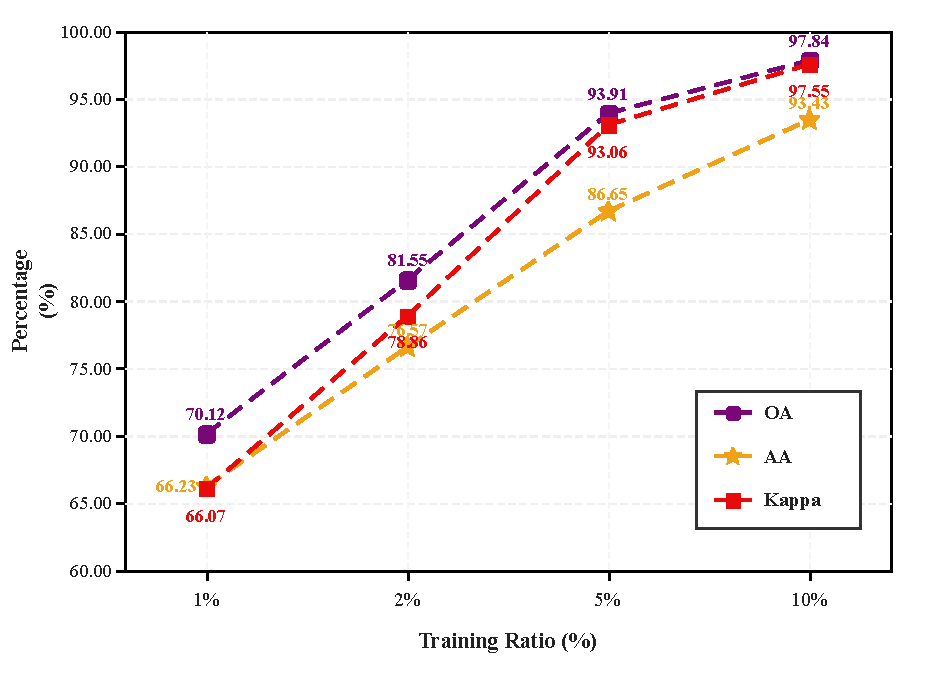
\includegraphics[width=0.325\textwidth]{figures/fig_scarcity_ip.pdf} &
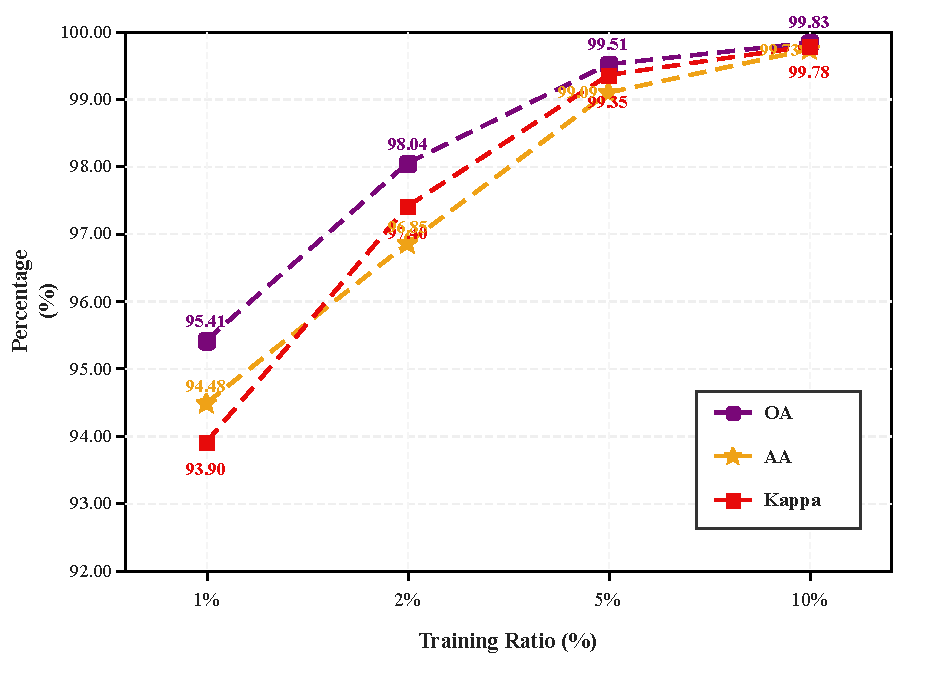
\includegraphics[width=0.325\textwidth]{figures/fig_scarcity_pu.pdf} &
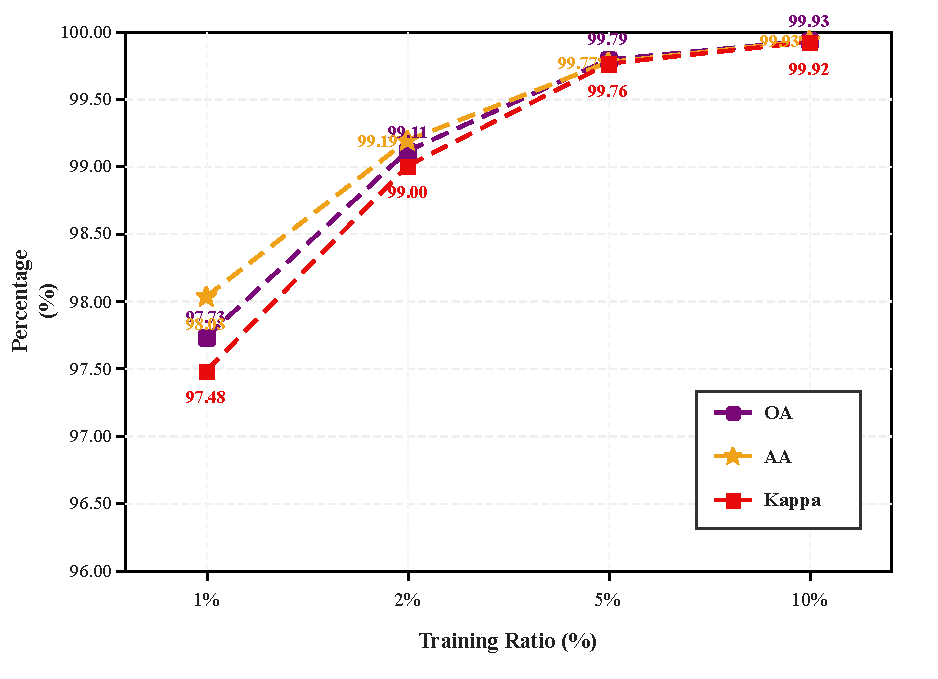
\includegraphics[width=0.325\textwidth]{figures/fig_scarcity_sv.pdf} \\
\footnotesize (a) Indian Pines & \footnotesize (b) Pavia University & \footnotesize (c) Salinas Valley \\
\end{tabular}
\caption{Performance degradation dynamics of SGSCF-Net under data scarcity stress testing across training ratios of 1\%, 2\%, 5\%, and 10\% on Indian Pines, Pavia University, and Salinas Valley. (a) Indian Pines. (b) Pavia University. (c) Salinas Valley.}
\label{fig:data_scarcity_degradation}
\Description{Performance degradation curves of SGSCF-Net under data scarcity across Indian Pines, Pavia University, and Salinas Valley.}
\end{figure*}

Fig.~\ref{fig:data_scarcity_degradation} illustrates the empirical performance degradation trajectories across the three benchmarks, while Table~\ref{tab:scarcity_table} reports the exact numerical metrics and percentage degradation.

\begin{table*}[t]
\centering
\footnotesize
\caption{Performance Degradation Analysis Under Data Scarcity Stress Testing Across Three Benchmarks (Patch $11 \times 11$, Batch 32, 200 Epochs).}
\label{tab:scarcity_table}
\begin{tabular*}{\textwidth}{@{\extracolsep{\fill}}lccccc}
\toprule
\textbf{Dataset Benchmark} & \textbf{1\% Train Ratio} & \textbf{2\% Train Ratio} & \textbf{5\% Train Ratio} & \textbf{10\% Train Ratio} & \textbf{Degradation (10\% $\to$ 1\%)} \\
\midrule
Indian Pines          & 70.12\% & 81.55\% & 93.91\% & 97.84\% & -27.73\% \\
Pavia University   & 95.41\% & 98.04\% & 99.51\% & 99.83\% & -4.43\% \\
Salinas Valley        & 97.73\% & 99.11\% & 99.79\% & 99.93\% & -2.20\% \\
\bottomrule
\end{tabular*}
\end{table*}

Table~\ref{tab:scarcity_table} and Fig.~\ref{fig:data_scarcity_degradation} expose distinct, dataset-specific sensitivity behaviors:
\begin{itemize}
    \item \textbf{Salinas Valley (-2.20\% drop):} As visualized in Fig.~\ref{fig:data_scarcity_degradation}, Salinas Valley exhibits exceptional resilience, retaining 97.73\% OA under a 1\% training ratio. Due to large contiguous fields and high intra-class spatial homogeneity, the SBAM and SCFG modules extract representative class descriptors even from minimal training patches.
    \item \textbf{Pavia University (-4.43\% drop):} Despite high intra-class spectral variance among urban materials, Pavia retains 95.41\% OA at 1\% training data. CBSA's complementary branch gating preserves distinct spectral signatures (such as Asphalt versus Bitumen) without confusing spatial edge transitions.
    \item \textbf{Indian Pines (-27.73\% drop):} Indian Pines experiences a steep performance decline from 97.84\% at 10\% down to 70.12\% at 1\%. As shown in Fig.~\ref{fig:data_scarcity_degradation}, a sharp degradation knee occurs below 5\% training ratio. This decline reflects a mathematical sample scarcity floor rather than an architectural defect, consistent with effective sample volume theory \cite{cui2019class} where representation quality degrades sharply when effective sample counts drop below class manifold rank.
\end{itemize}

\begin{table}[t]
\centering
\footnotesize
\caption{Class-Level Performance Extremes Under Extreme 1\% Training Scarcity.}
\label{tab:class_extremes_1percent}
\begin{tabular}{lll}
\toprule
\textbf{Dataset} & \textbf{Best Performing Class} & \textbf{Worst Performing Class} \\
\midrule
Indian Pines & Hay-windrowed (99.27\%) & Oats (7.66\%) \\
Pavia University & Painted metal sheets (99.62\%) & Self-Blocking Bricks (84.70\%) \\
Salinas Valley & Brocoli\_green\_weeds\_2 (100.00\%) & Fallow (89.47\%) \\
\bottomrule
\end{tabular}
\end{table}

Table~\ref{tab:class_extremes_1percent} details the per-dataset class extremes under 1\% data. On Indian Pines, the Oats category contains only 20 total labeled pixels across the entire scene. At a 1\% sampling ratio, the training set receives only $\max(\lfloor 0.01 \times 20 \rfloor, 3)$ or fewer than 2 distinct training patches. With only 1 or 2 patches available, learning high-dimensional 3D spatial-spectral features becomes mathematically indeterminate, dropping Oats accuracy to 7.66\%. Conversely, well-sampled categories such as Hay-windrowed maintain 99.27\% accuracy. Crucially, while baseline models such as SSAN collapse into predicting majority categories exclusively under this extreme regime, SGSCF-Net's minority-aware hybrid loss ($\mathcal{L}_{\text{Total}} = 0.7 \mathcal{L}_{\text{Spread}} + 0.3 \mathcal{L}_{\text{Focal}}$) prevents complete boundary collapse, preserving stable 70.12\% overall accuracy across the remaining fifteen categories, corroborating minority stabilization insights from prior imbalanced HSI literature \cite{cui2019class, haut2021generative, su2023spectral}.

\section{Conclusion and Future Work}
\label{sec:conclusion}
This article proposes the Spectral-Guided Spatial Cross-Attention Fusion Network (SGSCF-Net) to improve the classification performance and computational efficiency of hyperspectral image analysis. The architecture organically unifies input-level spectral gating, dual-stream convolutional feature extraction, and second-order spatial-channel pooling into an end-to-end framework. Specifically, the Spectral Band Attention Module (SBAM) dynamically attenuates atmospheric water-vapor noise on raw spectral bands before spatial convolution. The Complementary Branch Spectral Attention (CBSA) then enforces orthogonal feature specialization between pure-spectral ($1\times 1\times 7$) and joint spatial-spectral ($3\times 3\times 7$) 3D streams via complementary gating ($\alpha$ versus $1-\alpha$). Downstream, the Second-Order Covariance Fusion Gate (SCFG) replaces first-order global pooling with bilinear outer-product covariance pooling ($G = f_{\text{ch}} \otimes f_{\text{sp}}$), capturing localized spatial-channel co-activations while introducing only 82 learnable parameters. During training, a minority-aware hybrid objective ($\mathcal{L}_{\text{Spread}} + \mathcal{L}_{\text{Focal}}$) establishes margin-expanded decision boundaries to prevent representation collapse on severely imbalanced classes. Extensive experimental evaluations across Indian Pines, Pavia University, and Salinas Valley demonstrate that SGSCF-Net achieves competitive or superior accuracy (98.05\% OA and 94.82\% AA on Indian Pines, 99.82\% OA on Pavia University, and 99.92\% OA on Salinas Valley) while operating with only 308,097 parameters and an 8.80-minute training latency, successfully bypassing the quadratic computational constraints of Transformer self-attention.

In the future, based on the lightweight design of SGSCF-Net, we will investigate hardware-aware integer quantization (INT8/FP8) and structured tensor pruning to support onboard, real-time inference on edge NPUs and FPGAs aboard aerial and satellite platforms. We also plan to explore self-supervised masked spectral pre-training on large uncurated hyperspectral cubes to enhance representation transfer under extreme label scarcity. In addition, the second-order covariance fusion mechanism offers high architectural scalability for multimodal earth observation, providing a principled foundation for joint feature extraction and classification across co-registered hyperspectral and LiDAR data.

\begin{acks}
This research was conducted at the National Institute of Technology (NIT) Raipur. The authors express their gratitude to the NASA Jet Propulsion Laboratory and the Pavia University for providing the open-access hyperspectral benchmarks.
\end{acks}

\bibliographystyle{ACM-Reference-Format}
\bibliography{sample-base}

\end{document}
\endinput

